\section{Corrected Data}
\label{sec:GBJ1:FinalPlots}

In this section, the final plots that were shown in the publication are discussed. 
The plots shown are from  the leading \pt{} dijet selection and the forward/backwards selection and show the gap fraction as a function of \dy{}, \ptb{} and \qz{}, and also the mean number of jets in the rapidity interval as a function of \dy{} and \ptb{}. 
When \dy{} and \ptb{} are studied, \qz{} is always at a fixed value of 20 GeV. 
The data is sliced into different regions. 
The gap fraction and mean number of jets versus \dy{} distributions are shown for seven different \ptb{} ranges, and it is shown versus \ptb{} for five different \dy{} ranges. 
Each slice is offset to allow the data to be shown on one plot. 
The ratio of the theory predictions to data is shown next to each plot.

On each plot, the black points are the data points with statistical uncertainty bars, with the yellow bands indicating the systematic uncertainty from both the JES and unfolding. 
The red and blue dotted lines are the POWHEG + PYTHIA and POWHEG + HERWIG predictions respectively, and the blue band is the HEJ prediction with a theoretical uncertainty.

Figures \ref{GBJ1:dYSelA} and \ref{GBJ1:pTSelA} show the gap fraction and the ratio of theory to data as a function of $\dy{}$ and $\ptb{}$, respectively, for different \ptb{} and \dy{} slices for the leading \pt{} dijet selection. 
The gap fraction from the data reduces as a function of \ptb{} and \dy{}.
When the rapidity region between the dijets is small, the phase space for emission is small. 
When the \dy{} or the \ptb{} of the dijets increases, the phase space available for emission increase, and so the gap fraction decreases.
For the highest \ptb{} range, the gap fraction starts to level off. 
This feature could be due to PDF effects, where both of the jets have high \pt{}, and so the probability of having another jet in the event is low.
HEJ agrees well with the data for the complete range in $\dy$ for low $\ptb{}$. 
However, for $\ptb{}$ slices $150\le\ptb{}<180$ GeV and above, HEJ starts to overestimate the gap fraction.
This deviation is shown more clearly as a function of \ptb{}.
HEJ deviates from the data for $\ptb{}>140$ GeV for all but the highest \dy{} slices, in which there are significant uncertainties.
As described in Section \ref{Theory:MC}, HEJ is relevant only for hard wide angle emissions.
Therefore, is it not unexpected that it should do better when $\qz{}\approx\ptb{}$, and to do worse when $Q_{0}<<\ptb{}$.

POWHEG + PYTHIA and POWHEG + HERWIG give significantly different gap fractions as a function of \dy{} and \ptb{}.
POWHEG + PYTHIA gives the best overall description of the data.
POWHEG + PYTHIA agrees with the data at all \ptb{} slices for low \dy{}, however it starts to deviate for $\dy{}>3.5$. 
This can also be seen for the gap fraction as a function of \ptb{} for the different \dy{} slices. 
For the slices, $1\le\dy{}<2$, $2\le\dy{}<3$, and $3\le\dy{}<4$, the agreement is very good throughout \ptb{}, with only deviations away from the data at large \dy{} which correspond to statistical fluctuations.
However, for the other \dy{} slices POWHEG + PYTHIA gives too low a gap fraction.
Conversely, POWHEG + HERWIG only agrees with the data only in the lowest of \dy{} bins, it deviates for $\dy{}>1$ for all slices of \ptb{}. 
In the gap fraction against \ptb{} for different \dy{} slices distributions, POWHEG + HERWIG does not agree well with the data and underestimates the gap fraction for all considered regions of phase space.
The difference between POWHEG + PYTHIA and POWHEG + HERWIG is an indication of the uncertainty in current calculations of parton showers.


Figure \ref{GBJ1:Q0SelA} shows the gap fraction as a function of \qz{} for different slices in \dy{} and \ptb{} for the leading \pt{} dijet selection.
For a low \qz{} value, the gap fraction is at a minimum, as any increase in \qz{} will reduce the number of events with a jet above \qz{}.
When the \qz{} increases the gap fraction increases, which is expected as the probability of getting a very high \pt{} emission is lower.
POWHEG + HERWIG underestimates the data for all but the highest \qz{} bins, indicating that there is too much emission from the POWHEG + HERWIG parton shower. 
For the gap fraction against \qz{} for $2\le\dy{}<3$ and  $70\le\pt{}<90$ GeV slice, both HEJ and POWHEG + PYTHIA overlaps with the data throughout the \qz{} range. 
For the other slices, at low \qz{} HEJ overestimates the gap fraction, but improves as $\qz{}\approx\ptb{}$, which is expected as HEJ generates partons with similar \pt{}.
Neither POWHEG + PYTHIA or HEJ agrees well with the gap fraction when both \dy{} and \qz{} is large.



Figures \ref{GBJ1:NjetsdYSelA} and \ref{GBJ1:NjetspTSelA} are the mean number of jets in the rapidity interval between the boundary jets as a function of $\dy{}$ and $\ptb{}$, respectively, for slices in \ptb{} and \dy{} for the leading \pt{} dijet selection. 
This is an alternative method of probing the activity between the boundary jets. 
The gap fraction is only concerned with the leading jet in the rapidity region, but the average number of jets considers all jet in that region with a $\pt{}>20$ GeV. 
As with the gap fraction, POWHEG + PYTHIA agrees best with the data.
POWHEG + HERWIG consistently gives too much activity in the rapidity region, which helps to explain why the POWHEG + HERWIG gap fraction is below the data.
Except at very low \ptb{}, HEJ has too little activity in the rapidity region.
Comparing to the gap fraction slices, in which it agrees with data, would indicate that HEJ describes only the highest \pt{} emission between the dijet well. 

 
Figures \ref{GBJ1:dYSelB} and \ref{GBJ1:pTSelB} show the gap fraction and the ratio of theory to data as a function of $\dy{}$ and $\ptb{}$, respectively, for different \ptb{} and \dy{} slices for the forward/backward dijet selection.
For this selection, there are often imbalances in the \pt{} of the boundary jets, especially at larger \ptb{}.
All three model comparisons show similar difference to the data. 
The gap fraction from HEJ as a function of \dy{} falls below the data for low \ptb{} slices. 
It has been suggested in \cite{ref:Anderson1} that this is due to the importance of soft emission from the dijets.

Figure \ref{GBJ1:Q0SelB} shows the gap fraction as a function of \qz{} for different slices in \dy{} and \ptb{} for the forward/backward dijet selection.
In the leading \pt{} dijet selection, the maximum \pt{} of a jet in the rapidity region between the dijet system is the \pt{} of the subleading jet (which has a maximum \pt{} of \ptb{}).
Above the \ptb{} of the jet, the gap fraction must be one.
However, for the forward/backward dijet selection, the \pt{} of a jet in the rapidity region between the dijet system is less affected by the \ptb{}.
The gap fraction does not rise as quickly as in the previous selection.
The POWHEG + PYTHIA  shows similar agreement to the data as for the previous selection.
HEJ does not agree well with the data, and especially for the higher \dy{} slices, it has a consistently low gap fraction throughout \qz{}. 

Figure \ref{GBJ1:pTSelBQ0} shows the gap fraction as a function of $\dy{}$ and $\ptb{}$ respectively for different \ptb{} and \dy{} slices for the forward/backward dijet selection, but the \qz{} is set to the \ptb{} of the event. 
This shows how the gap fraction is affected by emissions which are harder than the \ptb{} of the  dijets. 
POWHEG + PYTHIA and POWHEG + HERWIG both overlap the data.
This would indicate that this definition of the gap fraction is less dependent on the modelling of the parton shower, hadronisation and underlying event.
The new definition of the jet veto does not improve the HEJ agreement with the data.


Since publishing the results of this analysis, several papers \cite{ref:Anderson1,ref:JeffNew} have compared  their theoretical predictions to the ATLAS data. 
Both discuss the unreliability of fixed order calculations in this topology of event.
Reference \cite{ref:JeffNew} uses an all-order resummation in $\ln(\pt{}/\qz{})$ terms to compare to the data, observing a large theoretical uncertainty. 
The conclusion of the paper is: ``The message is clear: the accuracy of the ATLAS data already demands better theoretical calculations''.


\begin{figure}
\centering
        \begin{subfigure}[b]{0.5\textwidth}
                \centering
                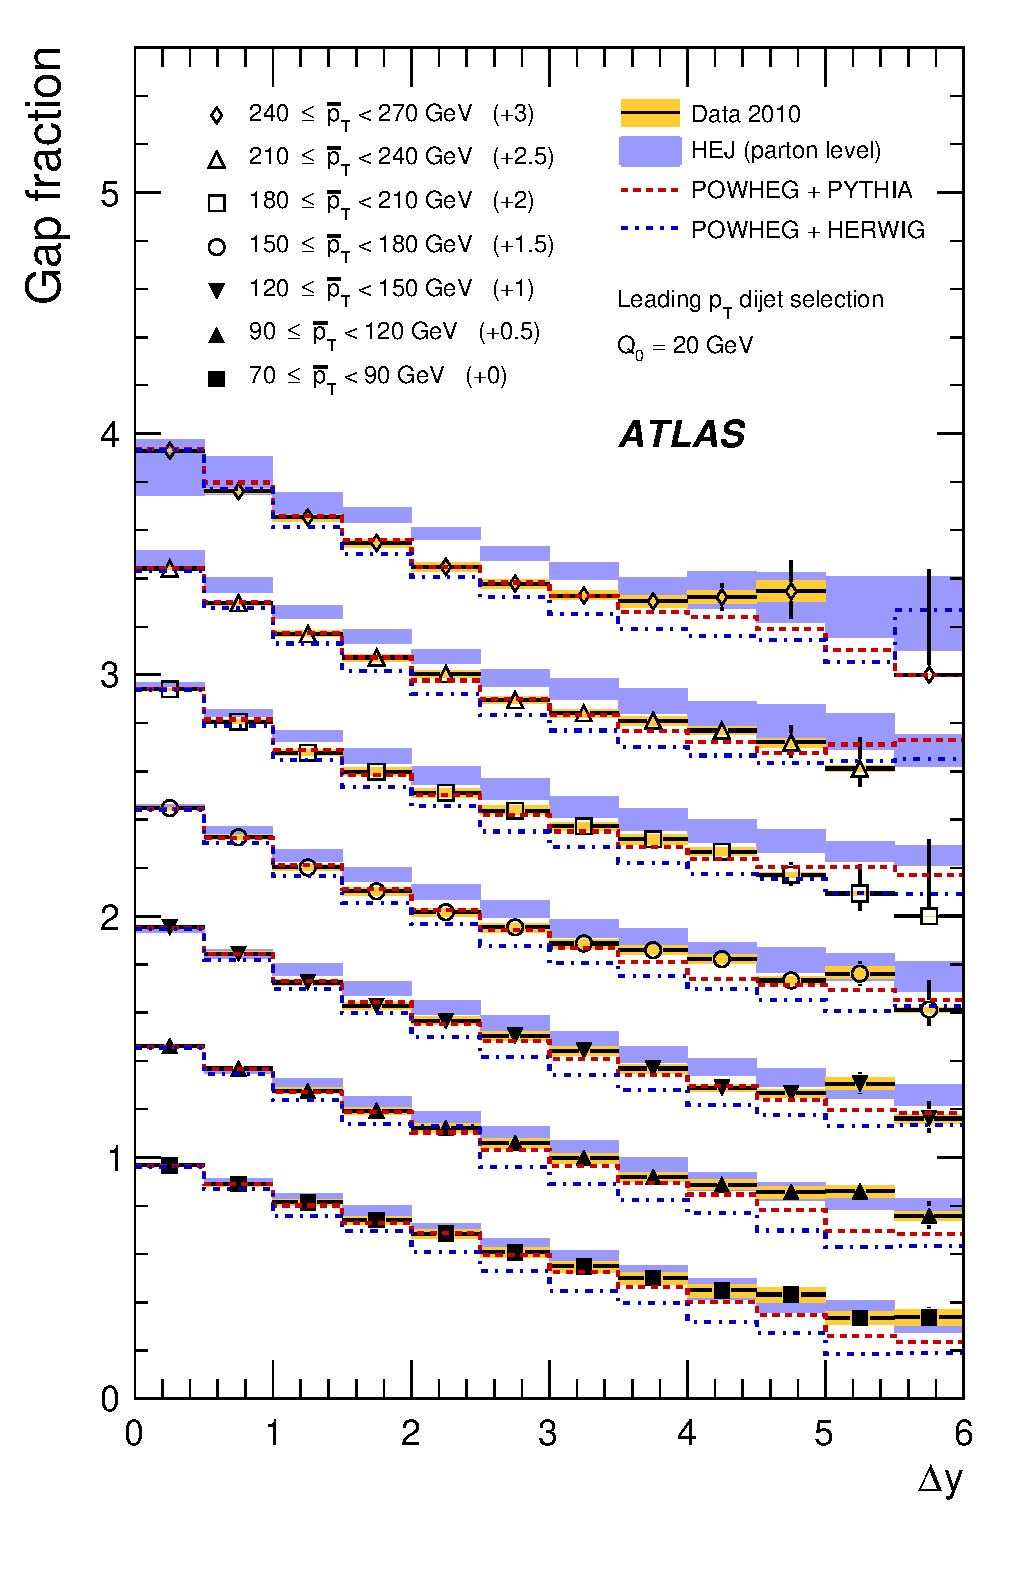
\includegraphics[width=\textwidth]{figures/GBJ1/FinalData/GF_dY.eps}
        \end{subfigure}%
        \begin{subfigure}[b]{0.5\textwidth}
                \centering
                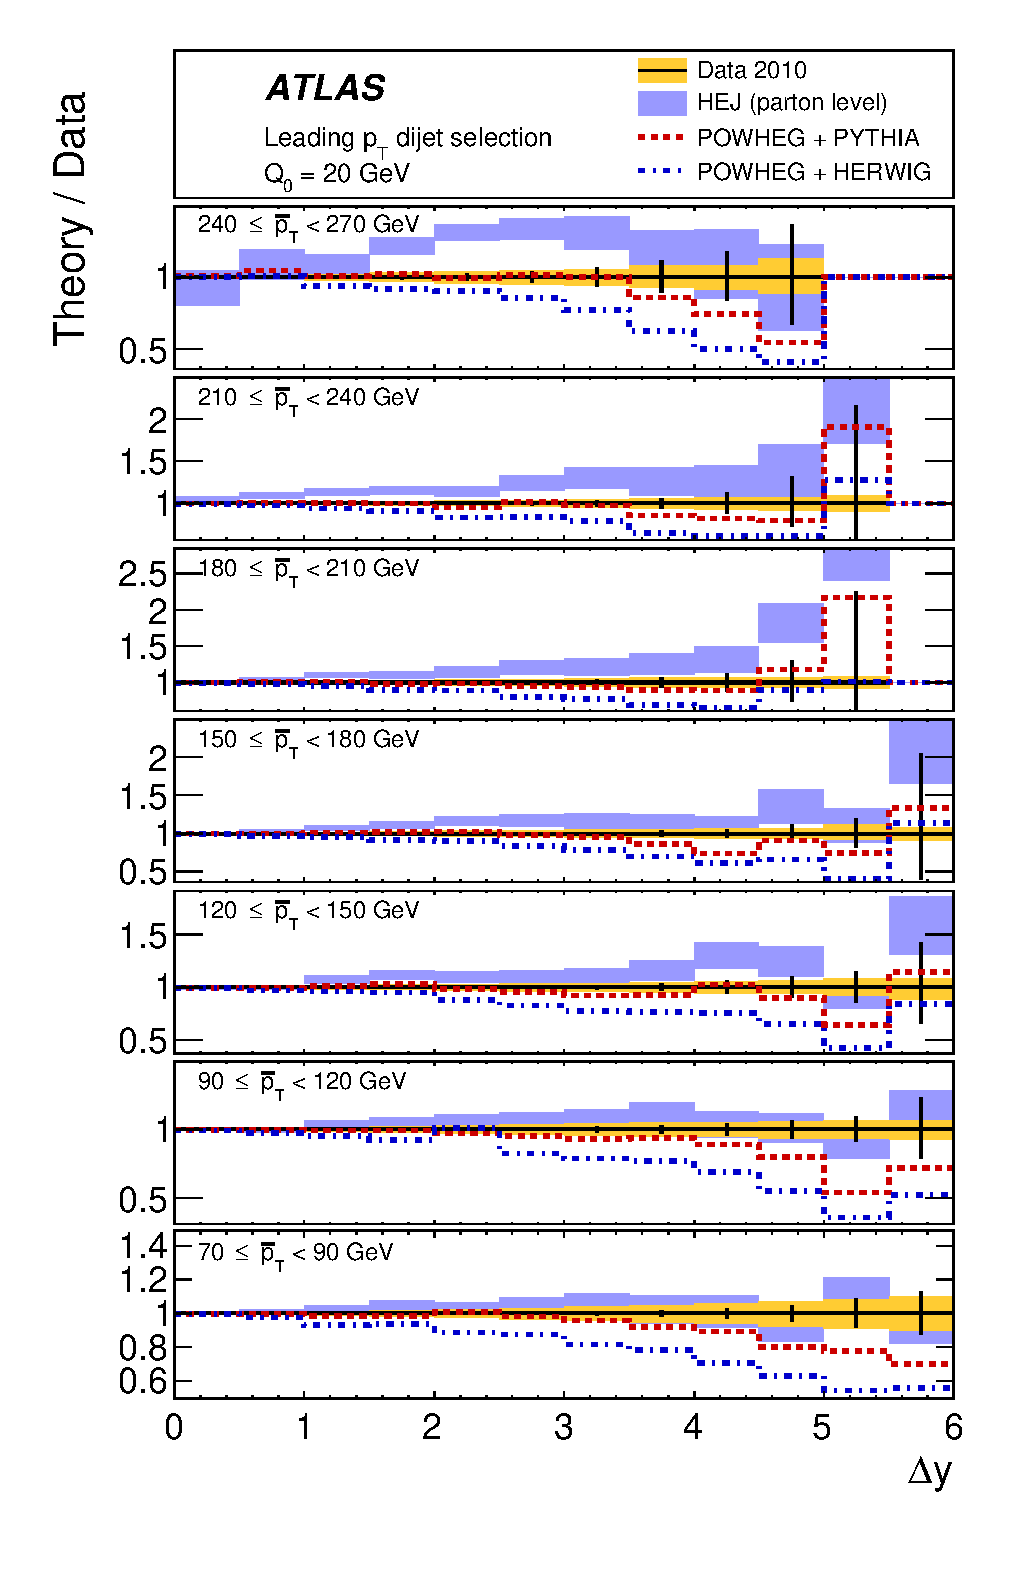
\includegraphics[width=\textwidth]{figures/GBJ1/FinalData/GF_dY_ratio.eps}
        \end{subfigure}%

        \begin{subfigure}[b]{0.5\textwidth}
                \centering
                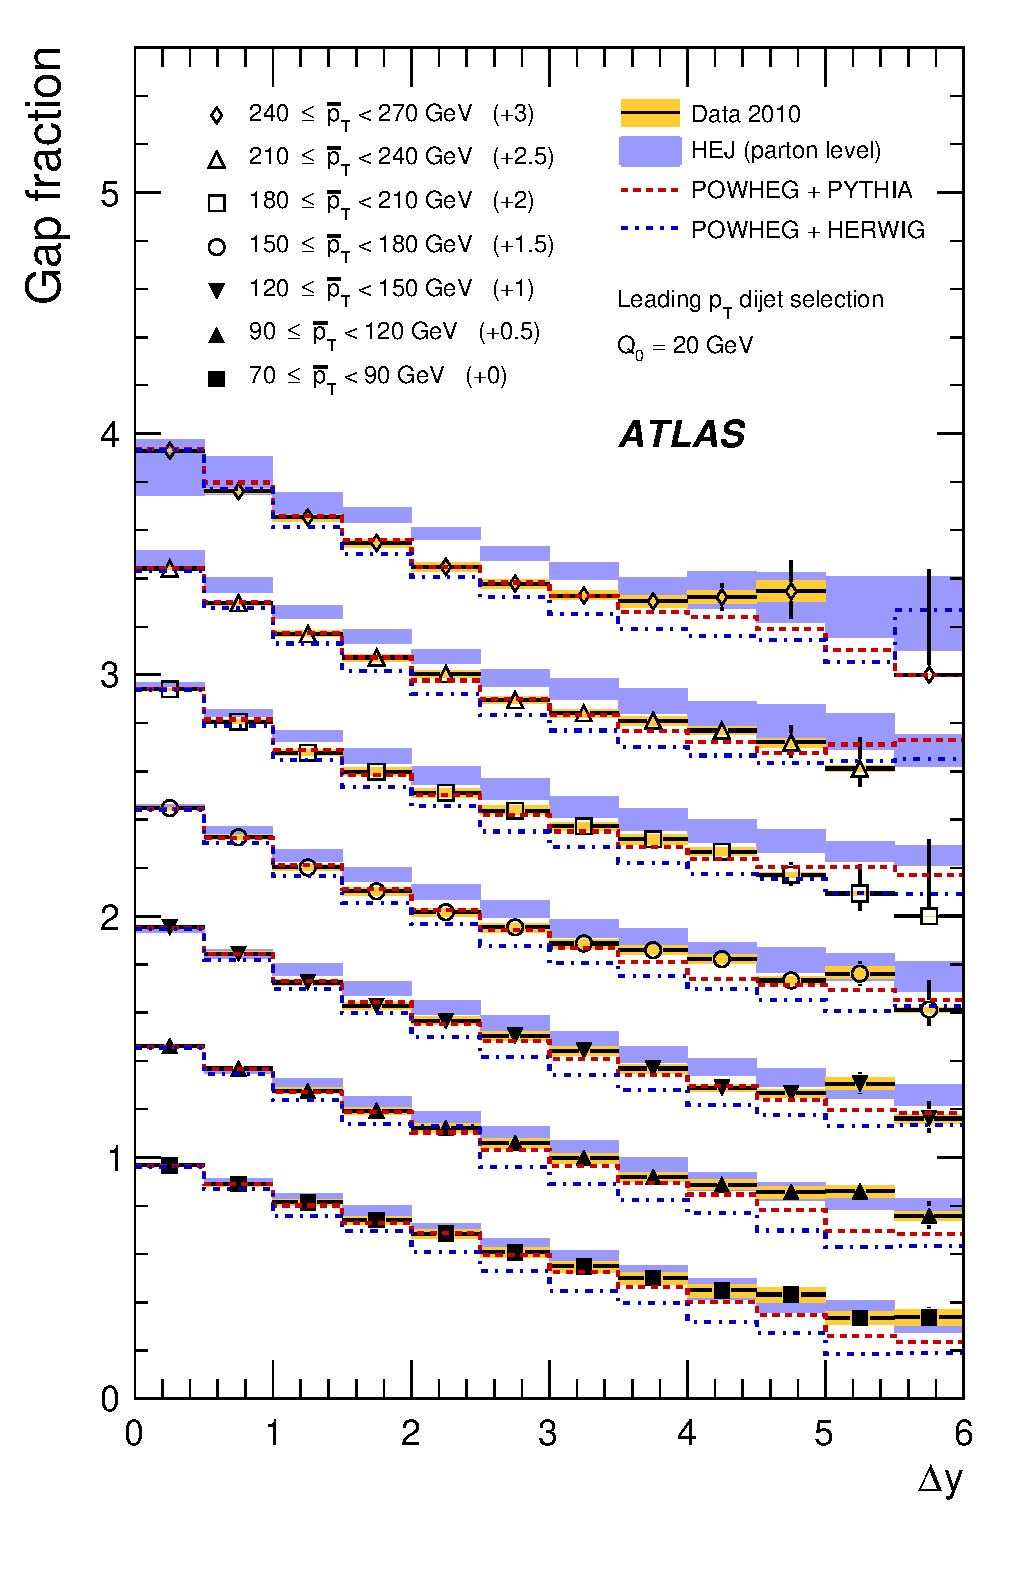
\includegraphics[width=\textwidth]{figures/GBJ1/FinalData/GF_dY.eps}
        \end{subfigure}%
        \begin{subfigure}[b]{0.5\textwidth}
                \centering
                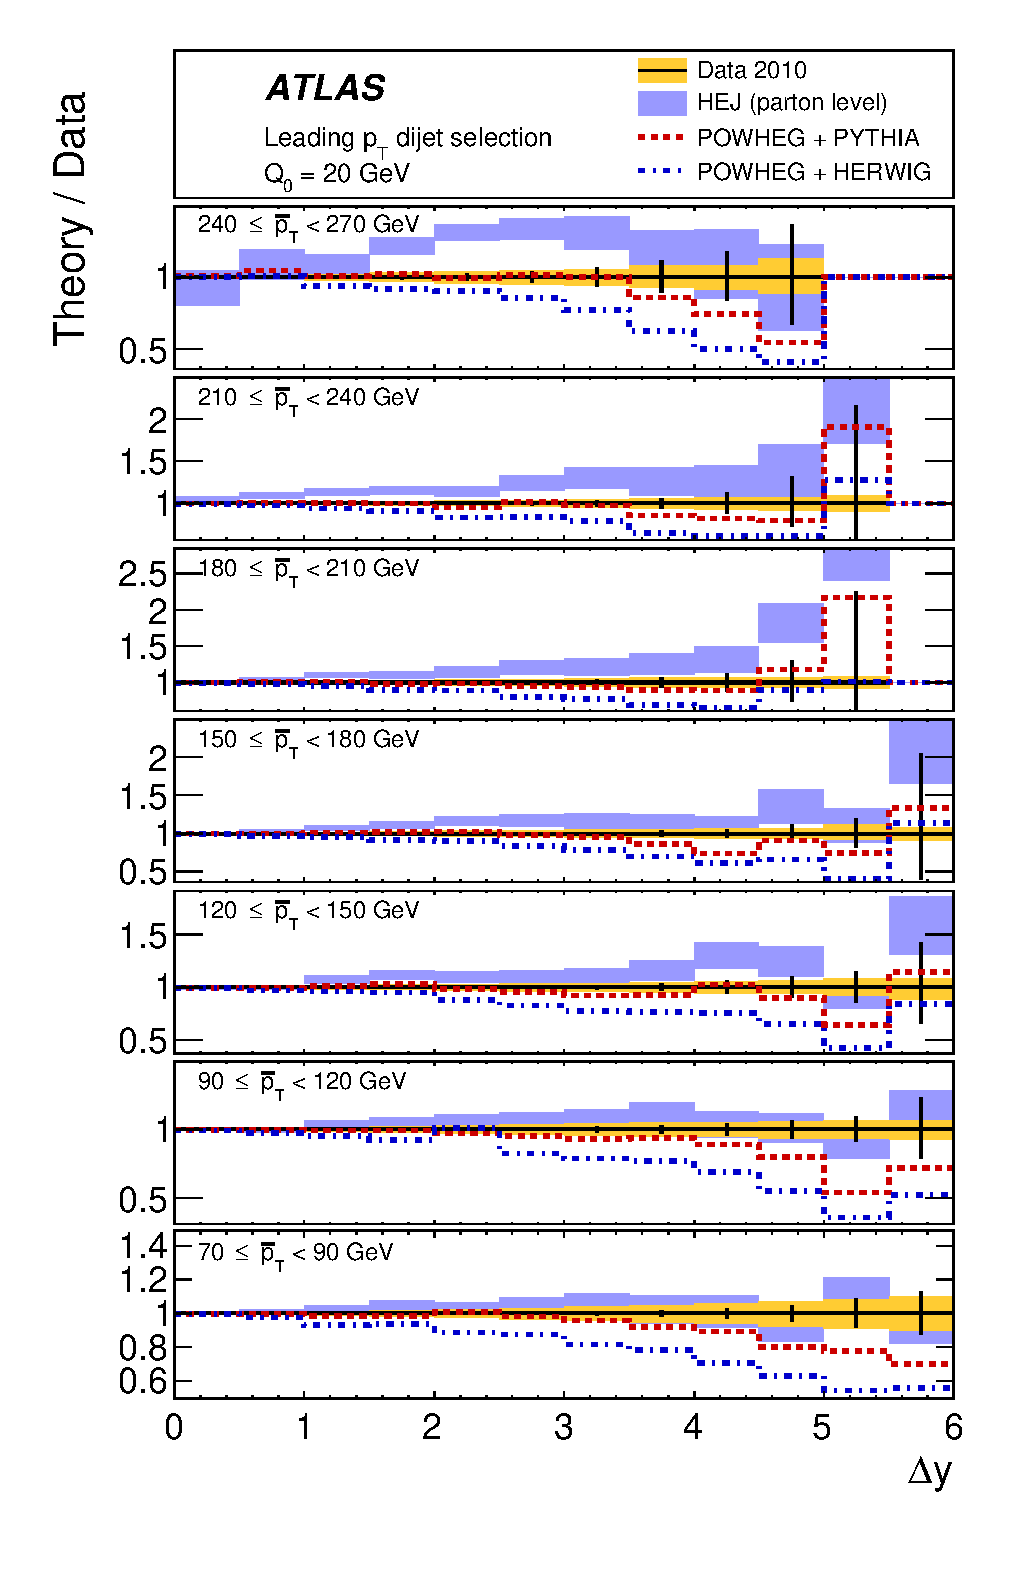
\includegraphics[width=\textwidth]{figures/GBJ1/FinalData/GF_dY_ratio.eps}
        \end{subfigure}%
\caption[Gap fraction as a function of  \dy{} for the leading \pt{} dijet selection]{
(a) Gap fraction as a function of \dy{} for various \ptb{} slices for the leading \pt{} dijet selection. 
(b) Ratio between the theoretical predictions and the data.
\label{GBJ1:dYSelA}}
\end{figure}



\begin{figure}
\centering
        \begin{subfigure}[b]{0.5\textwidth}
                \centering
                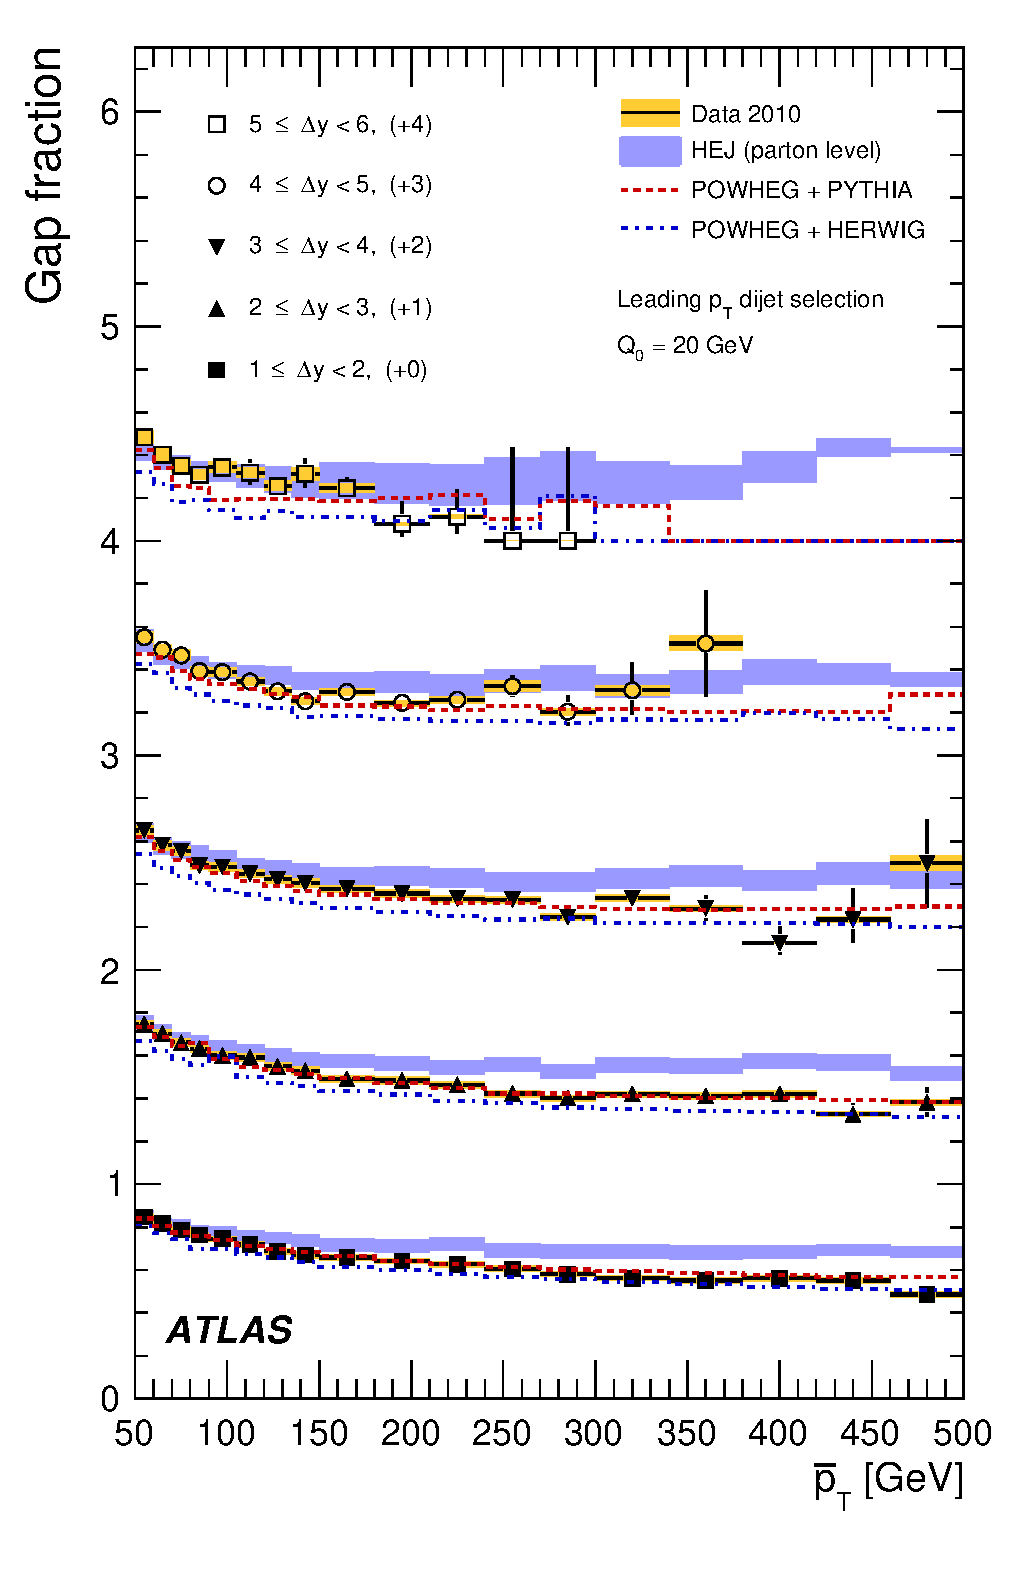
\includegraphics[width=\textwidth]{figures/GBJ1/FinalData/GF_ptBar.eps}
        \end{subfigure}%
        \begin{subfigure}[b]{0.5\textwidth}
                \centering
                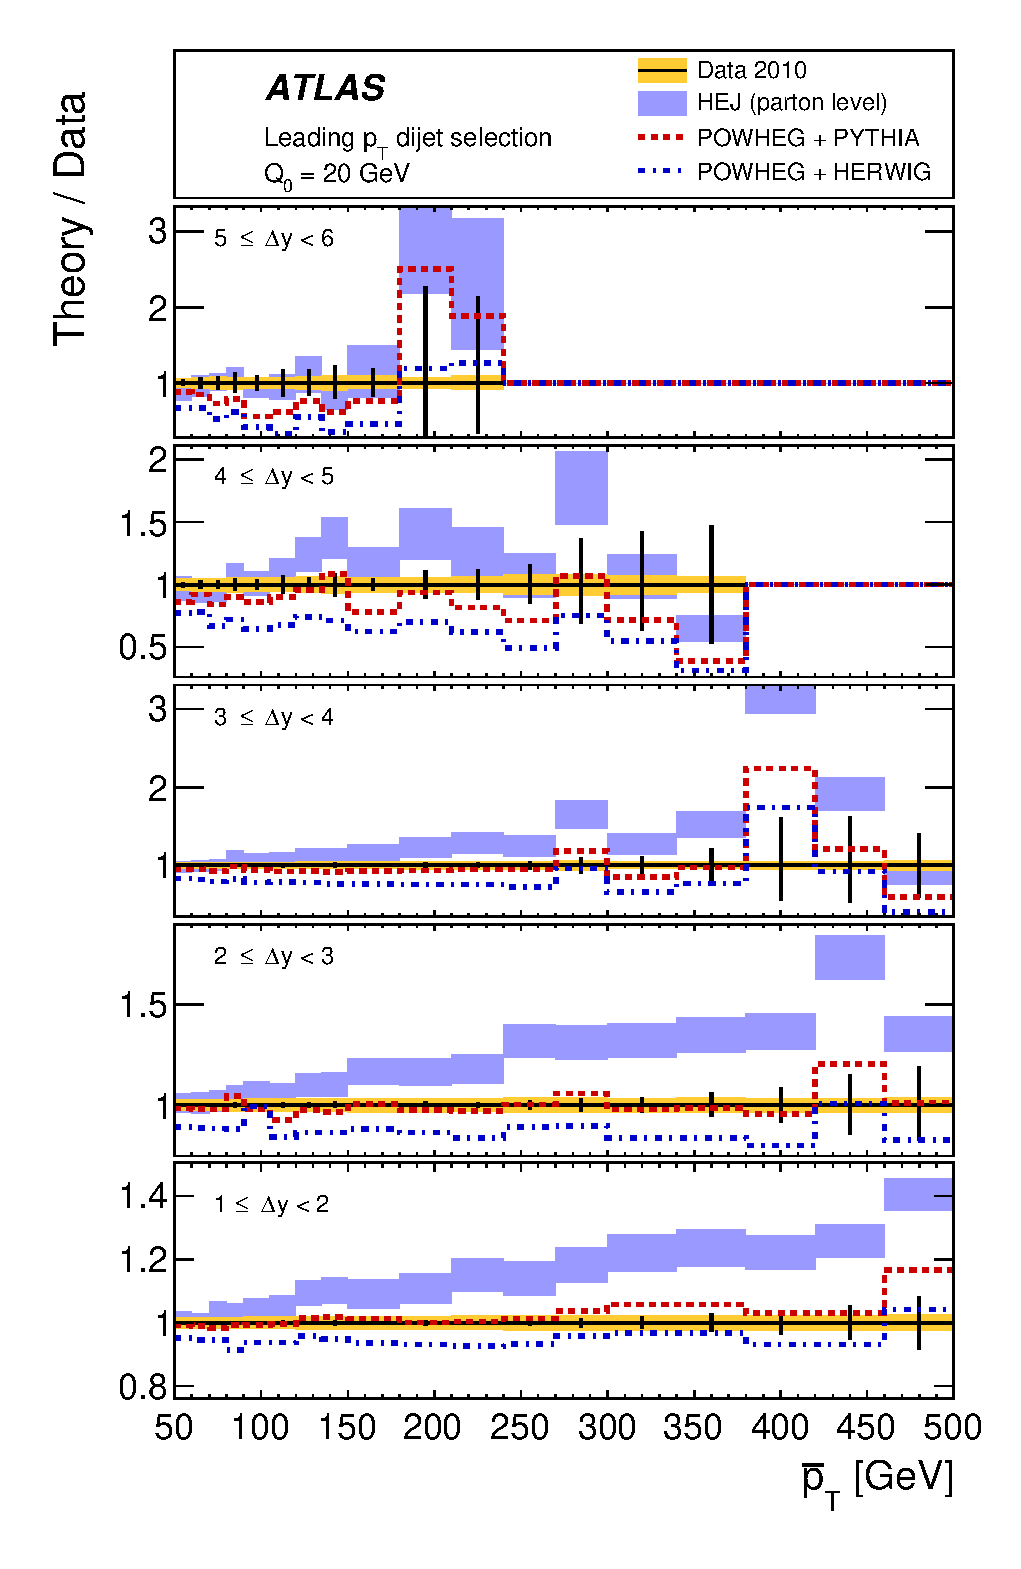
\includegraphics[width=\textwidth]{figures/GBJ1/FinalData/GF_ptBar_ratio.eps}
        \end{subfigure}%
\caption[Gap fraction as a function of \ptb{} for leading \pt{} dijet selection]{ 
(a) Gap fraction as a function of \ptb{} for various \dy{} slices for the leading \pt{} dijet selection. 
(b) Ratio between the theoretical predictions and data.
\label{GBJ1:pTSelA}}
\end{figure}



\begin{figure}
\centering
        \begin{subfigure}[b]{0.5\textwidth}
                \centering
                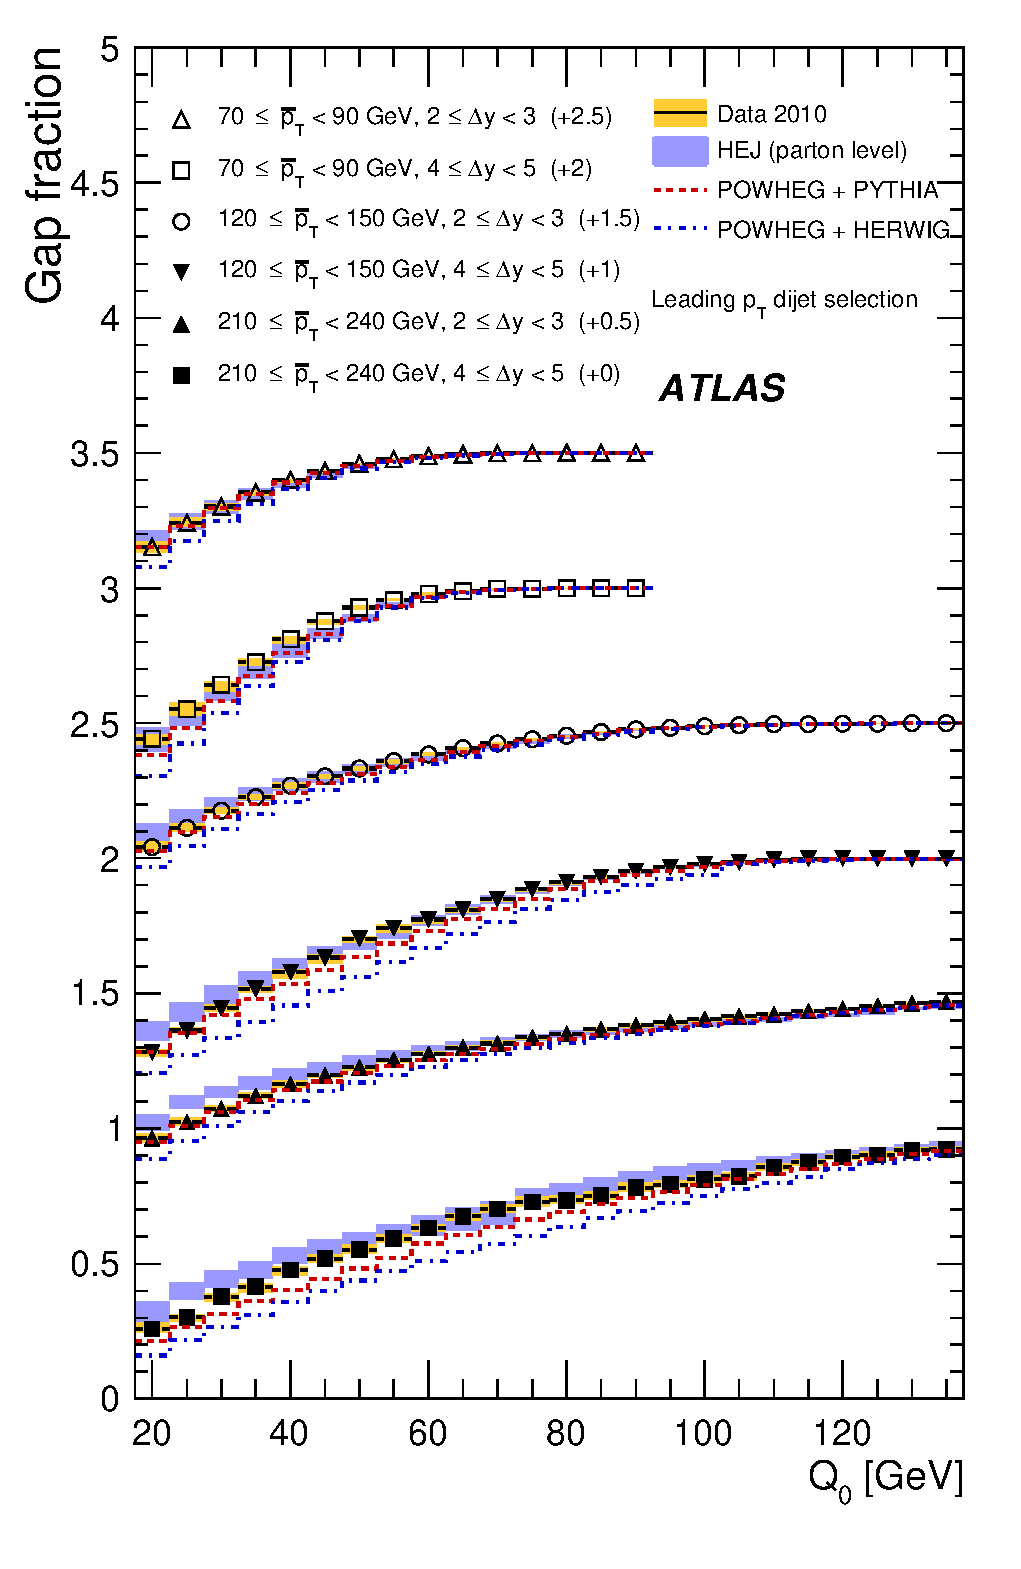
\includegraphics[width=\textwidth]{figures/GBJ1/FinalData/GF_Q0.eps}
        \end{subfigure}%
        \begin{subfigure}[b]{0.5\textwidth}
                \centering
                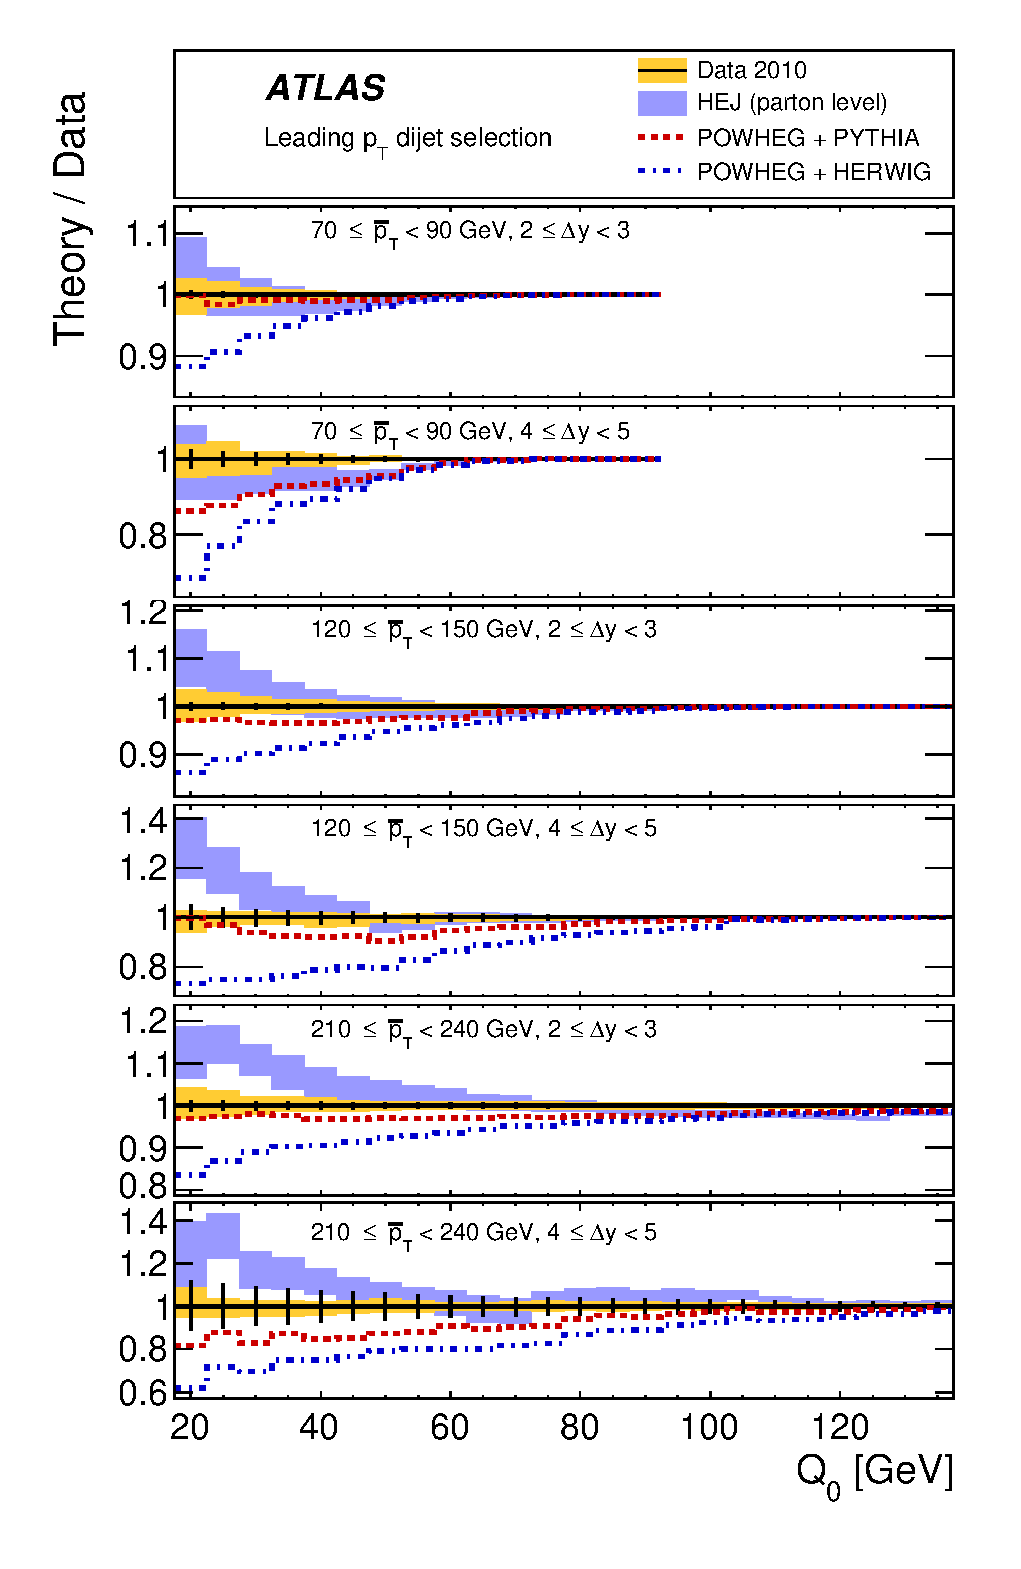
\includegraphics[width=\textwidth]{figures/GBJ1/FinalData/GF_Q0_ratio.eps}
        \end{subfigure}%
\caption[Gap fraction as a function of \qz{} for leading \pt{} dijet selection]{ 
(a) Gap fraction as a function of \qz{} for various \dy{} and \ptb{} slices for the leading \pt{} dijet selection. 
(b) Ratio between the theoretical predictions and data. 
\label{GBJ1:Q0SelA}}
\end{figure}

\begin{figure}
\centering
        \begin{subfigure}[b]{0.5\textwidth}
                \centering
                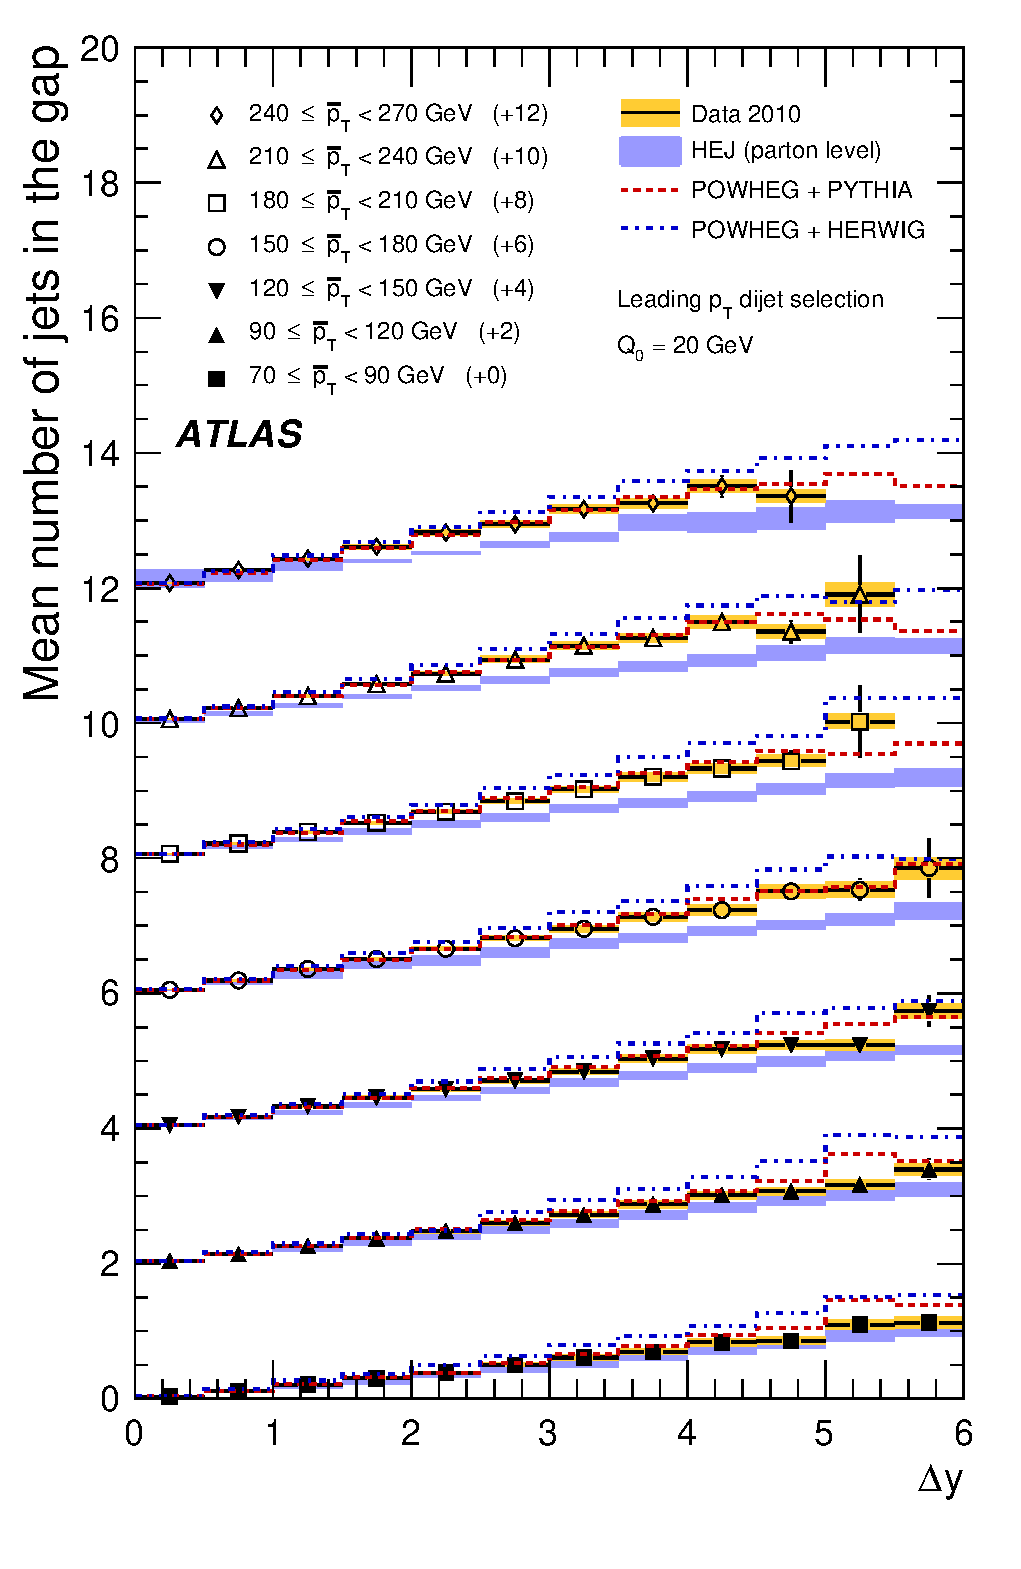
\includegraphics[width=\textwidth]{figures/GBJ1/FinalData/GF_Njets_dY.eps}
        \end{subfigure}%
        \begin{subfigure}[b]{0.5\textwidth}
                \centering
                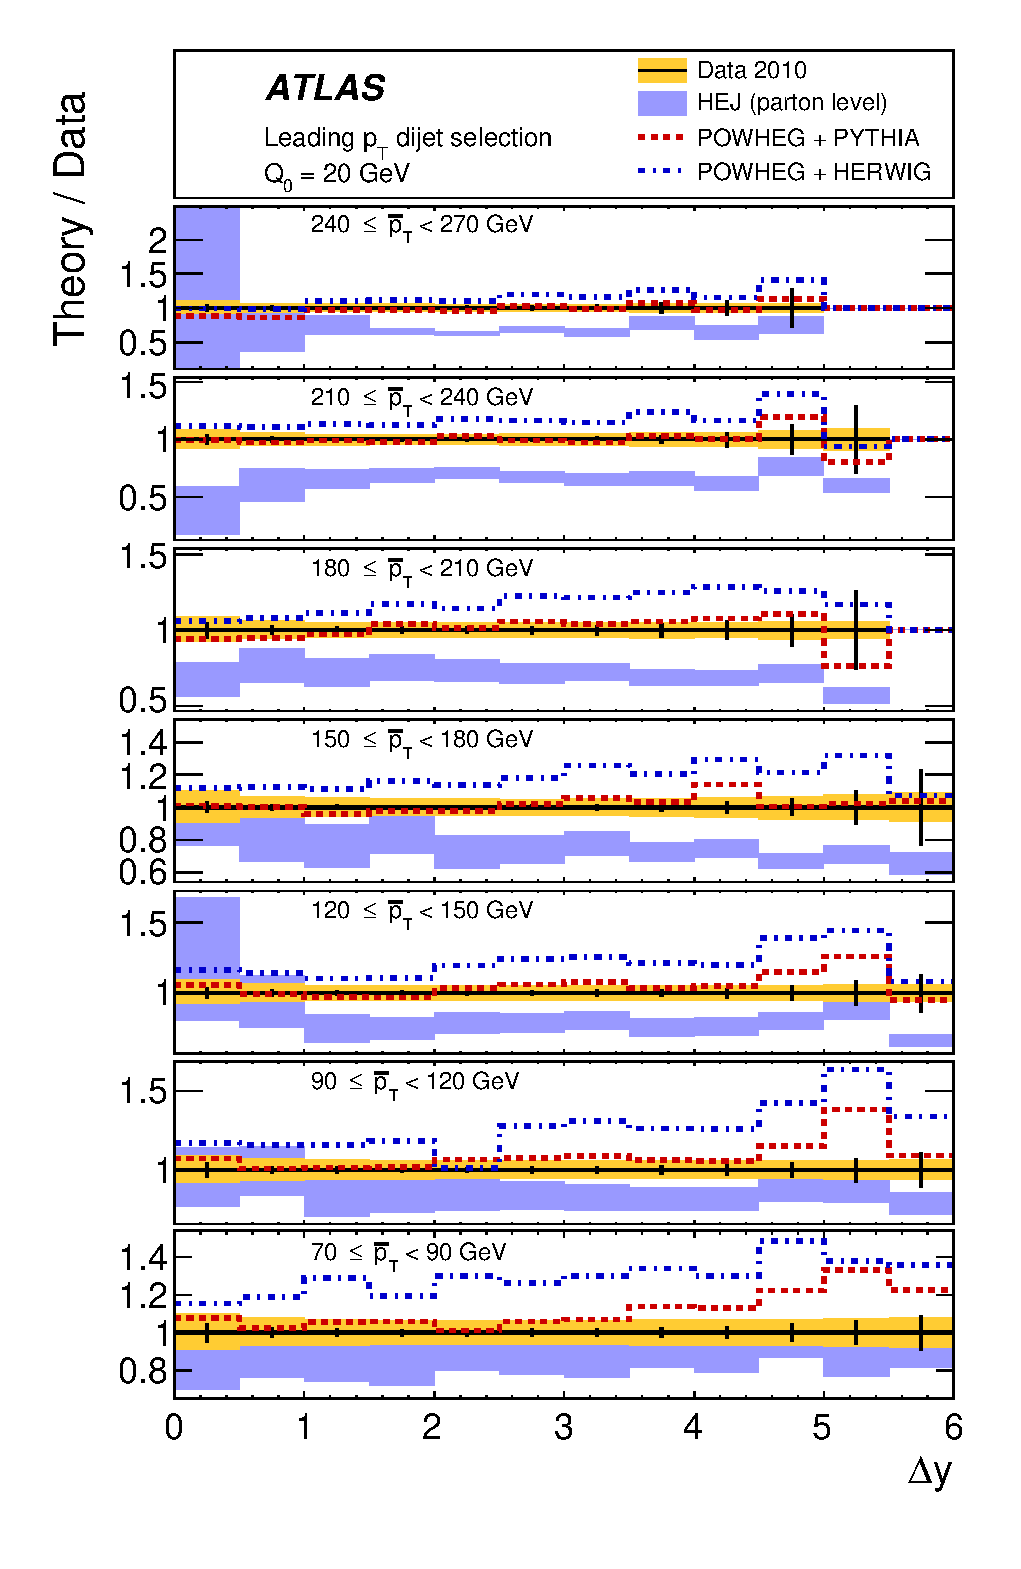
\includegraphics[width=\textwidth]{figures/GBJ1/FinalData/GF_Njets_dY_ratio.eps}
        \end{subfigure}%
\caption[Mean number of jets as a function of \dy{} for leading \pt{} dijet selection]{ 
(a) Mean number of jets in the rapidity region bounded by the dijet system as a function of \dy{} for various \ptb{} slices for the leading \pt{} dijet selection. 
(b) Ratio between the theoretical predictions and data. 
\label{GBJ1:NjetsdYSelA}}
\end{figure}

\begin{figure}
\centering
        \begin{subfigure}[b]{0.5\textwidth}
                \centering
                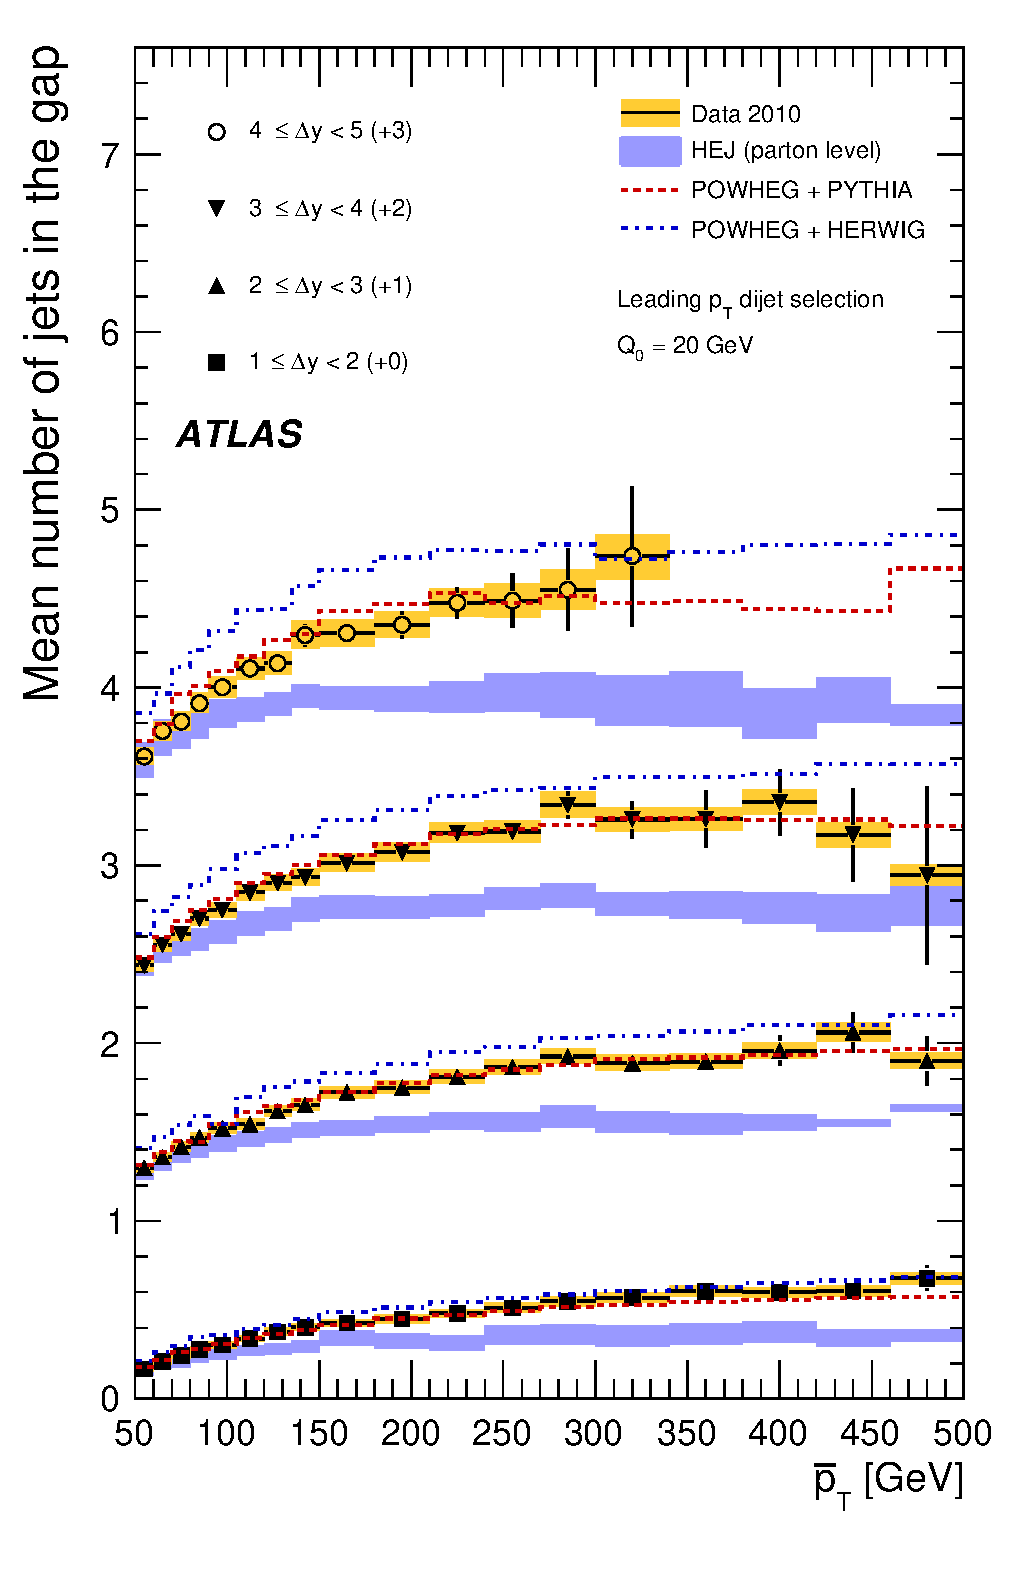
\includegraphics[width=\textwidth]{figures/GBJ1/FinalData/GF_Njets.eps}
        \end{subfigure}%
        \begin{subfigure}[b]{0.5\textwidth}
                \centering
                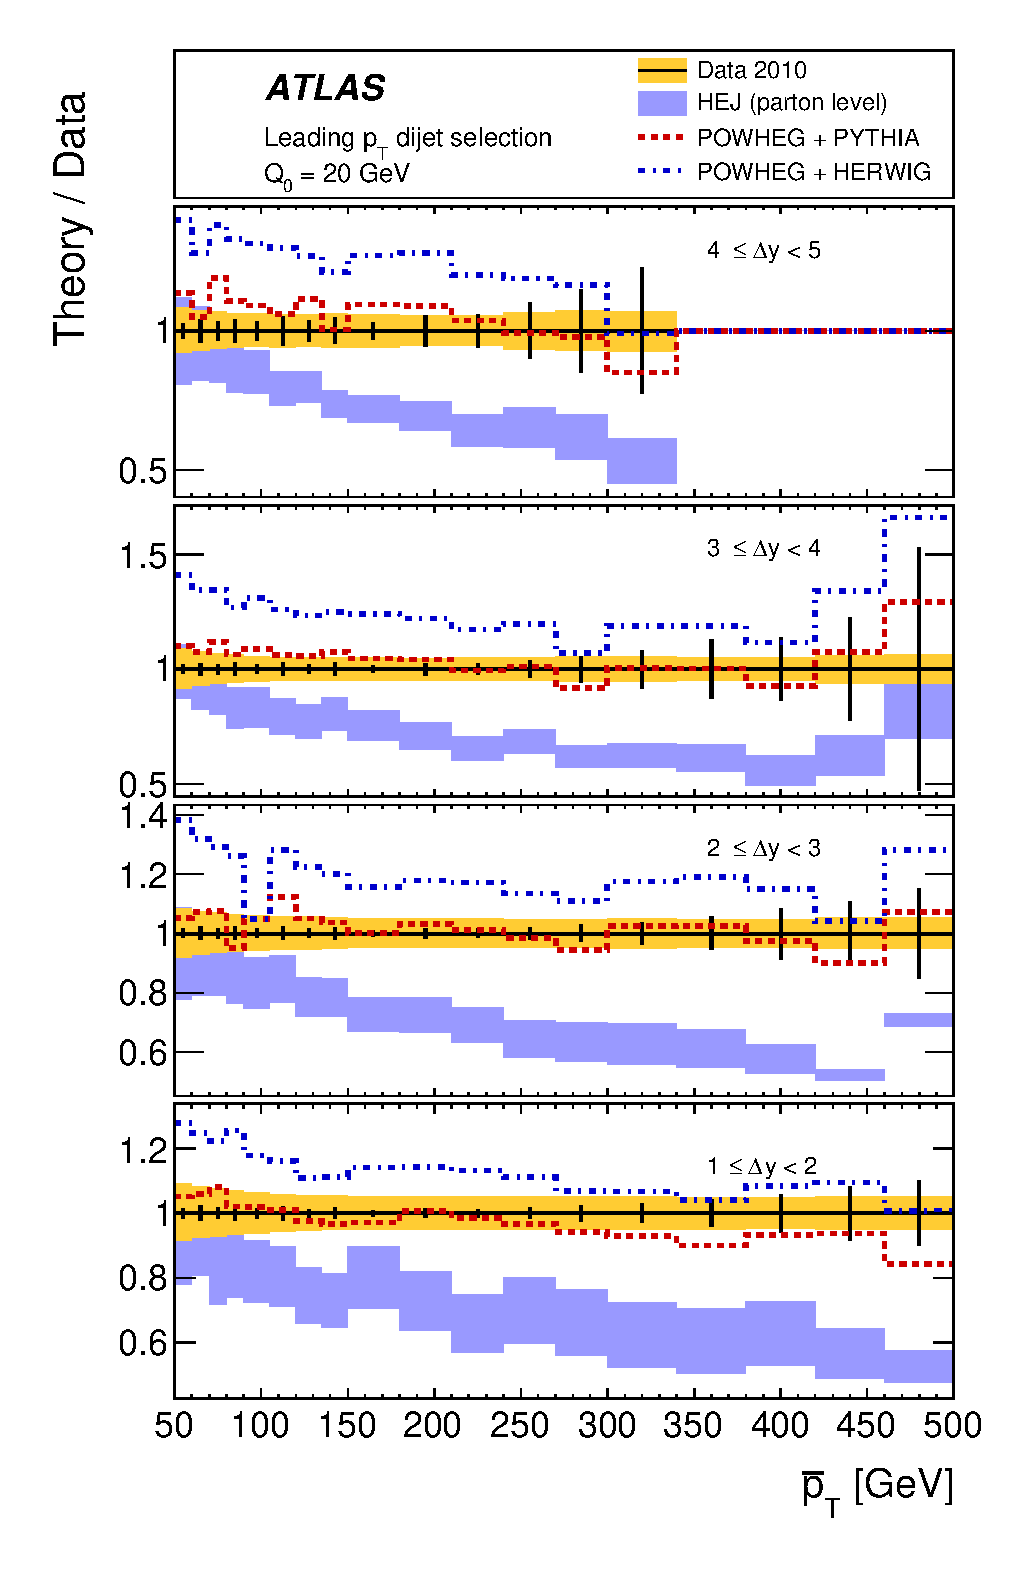
\includegraphics[width=\textwidth]{figures/GBJ1/FinalData/GF_Njets_ratio.eps}
        \end{subfigure}%
\caption[Mean number of jets as a function of \ptb{} for leading $p_T$ dijet selection]{ 
(a) Mean number of jets in the rapidity region bounded by the dijet system as a function of \ptb{} for various \dy{} slices for the leading \pt{} dijet selection. 
(b) Ratio between the theoretical predictions and data.
\label{GBJ1:NjetspTSelA}}
\end{figure}

%%%%%%%%%%%%%%%%%%%SELECTION B%%%%%%%%%%%%%%%%%%%%%%

\begin{figure}
\centering
        \begin{subfigure}[b]{0.5\textwidth}
                \centering
                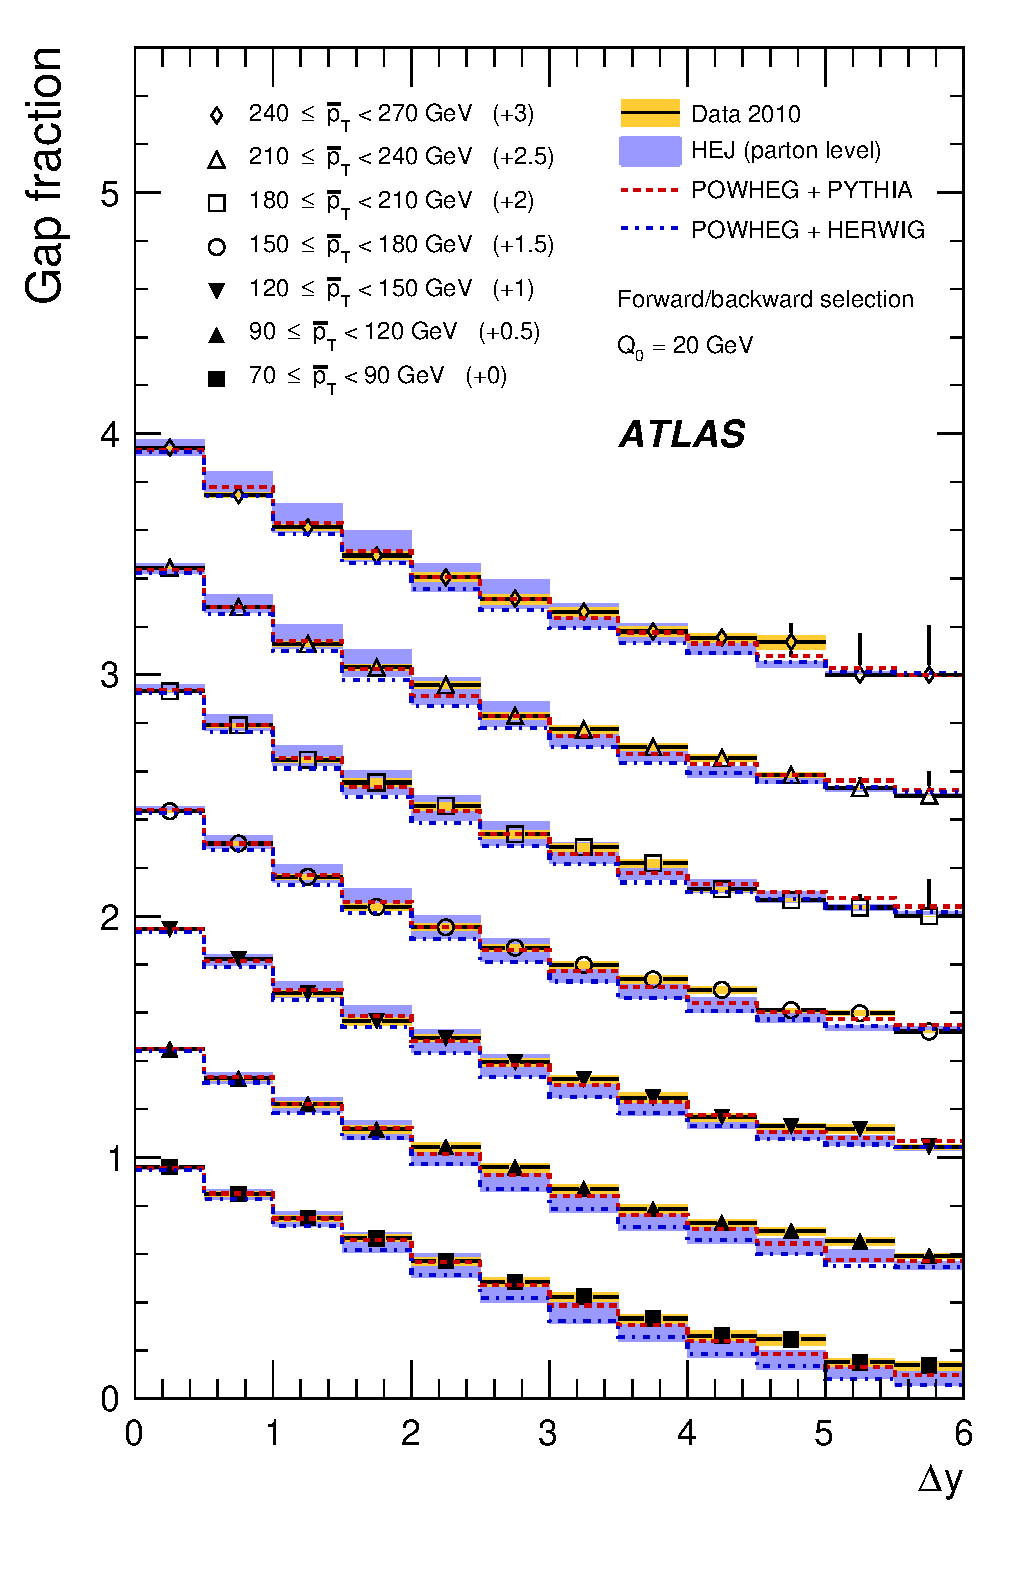
\includegraphics[width=\textwidth]{figures/GBJ1/FinalData/GF_dY_SelB.eps}
        \end{subfigure}%
        \begin{subfigure}[b]{0.5\textwidth}
                \centering
                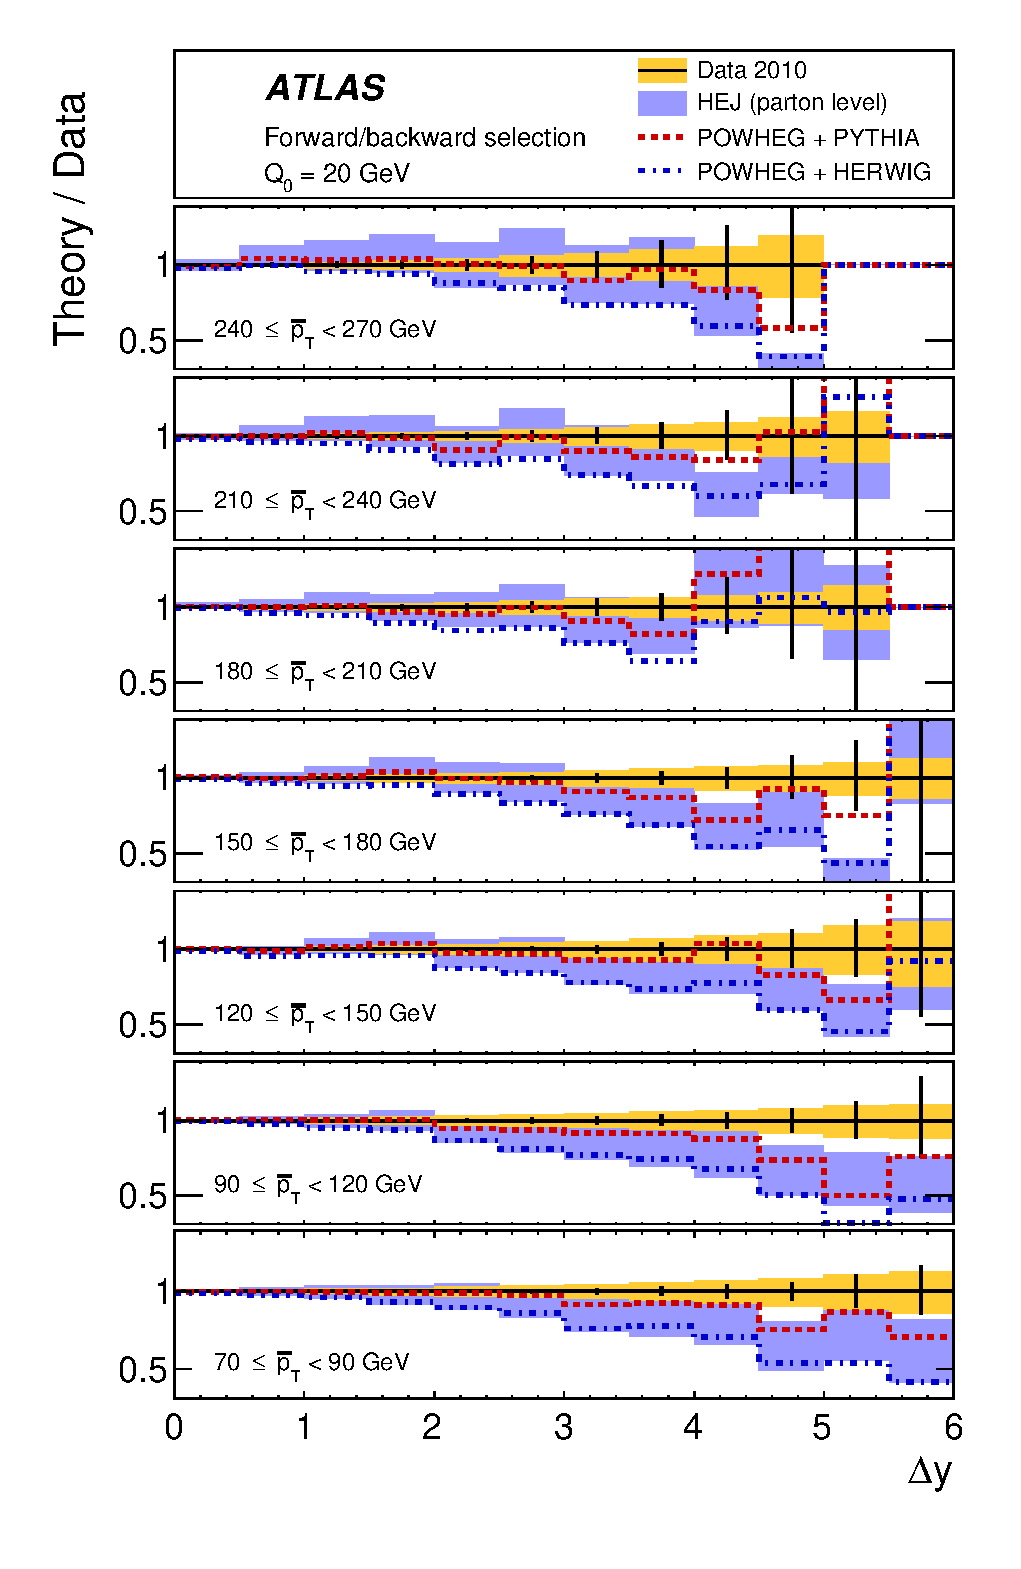
\includegraphics[width=\textwidth]{figures/GBJ1/FinalData/GF_dY_SelB_ratio.eps}
        \end{subfigure}%
\caption[Gap fraction as a function of \dy{} for forward backward selection]{ 
(a) Gap fraction as a function of \dy{} for various \ptb{} slices for the forward backward selection. 
(b) Ratio between the theoretical predictions and data. 
\label{GBJ1:dYSelB}}
\end{figure}

\begin{figure}
\centering
        \begin{subfigure}[b]{0.5\textwidth}
                \centering
                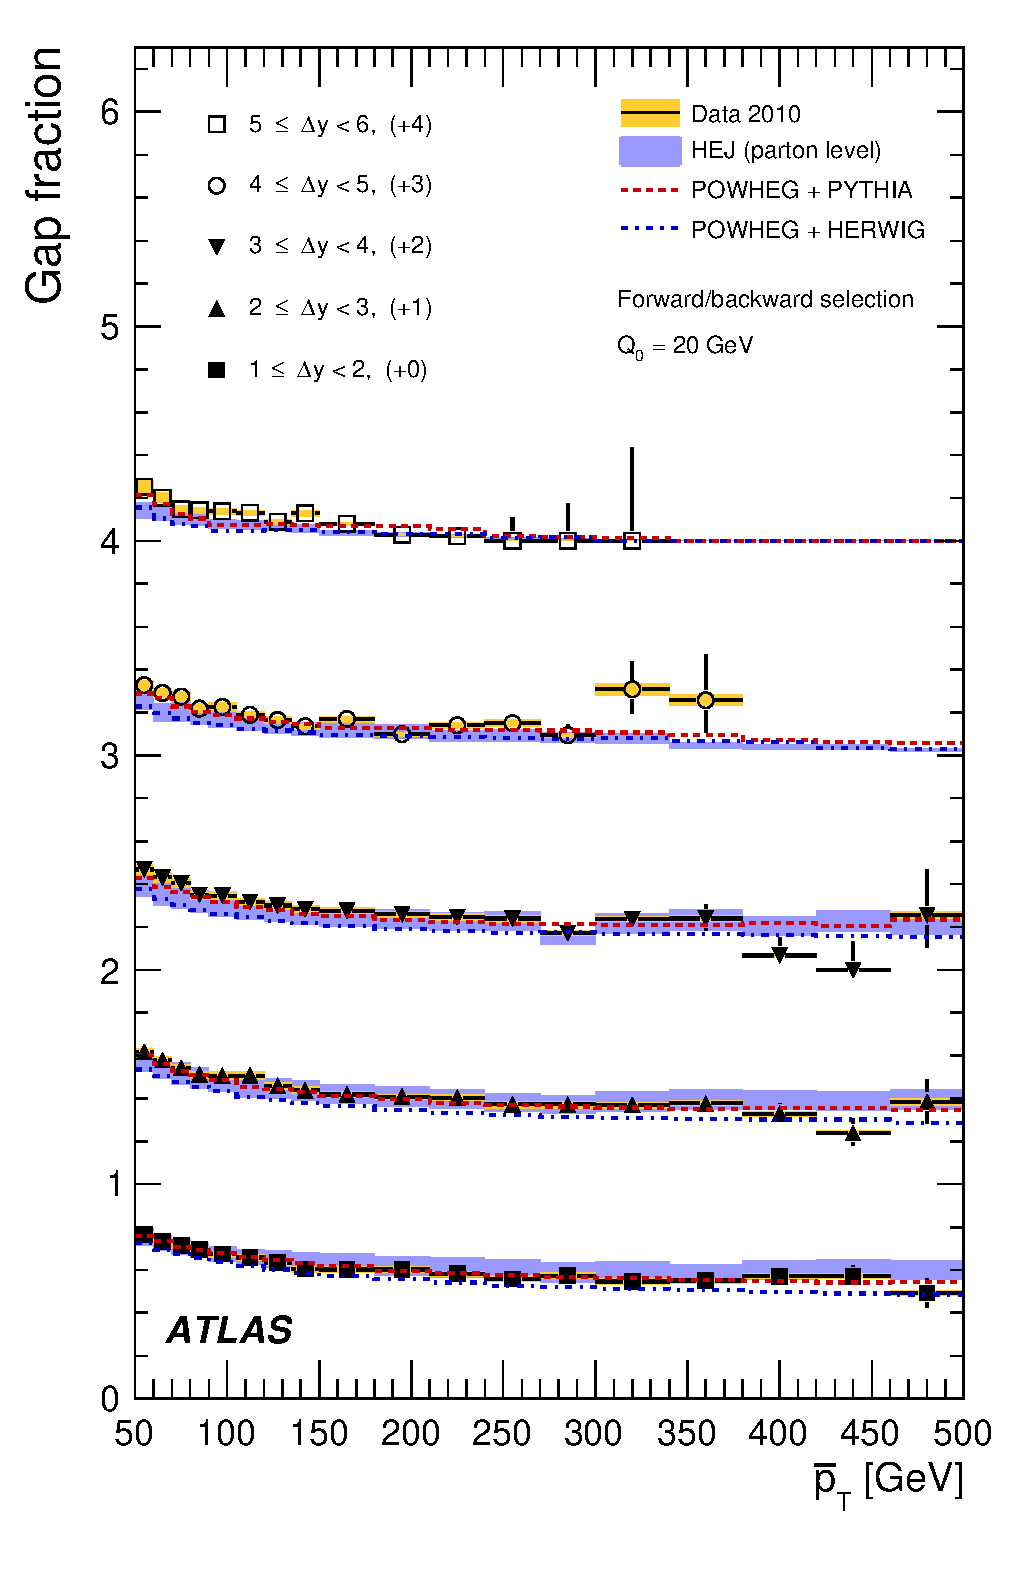
\includegraphics[width=\textwidth]{figures/GBJ1/FinalData/GF_SelB_pT.eps}
        \end{subfigure}%
        \begin{subfigure}[b]{0.5\textwidth}
                \centering
                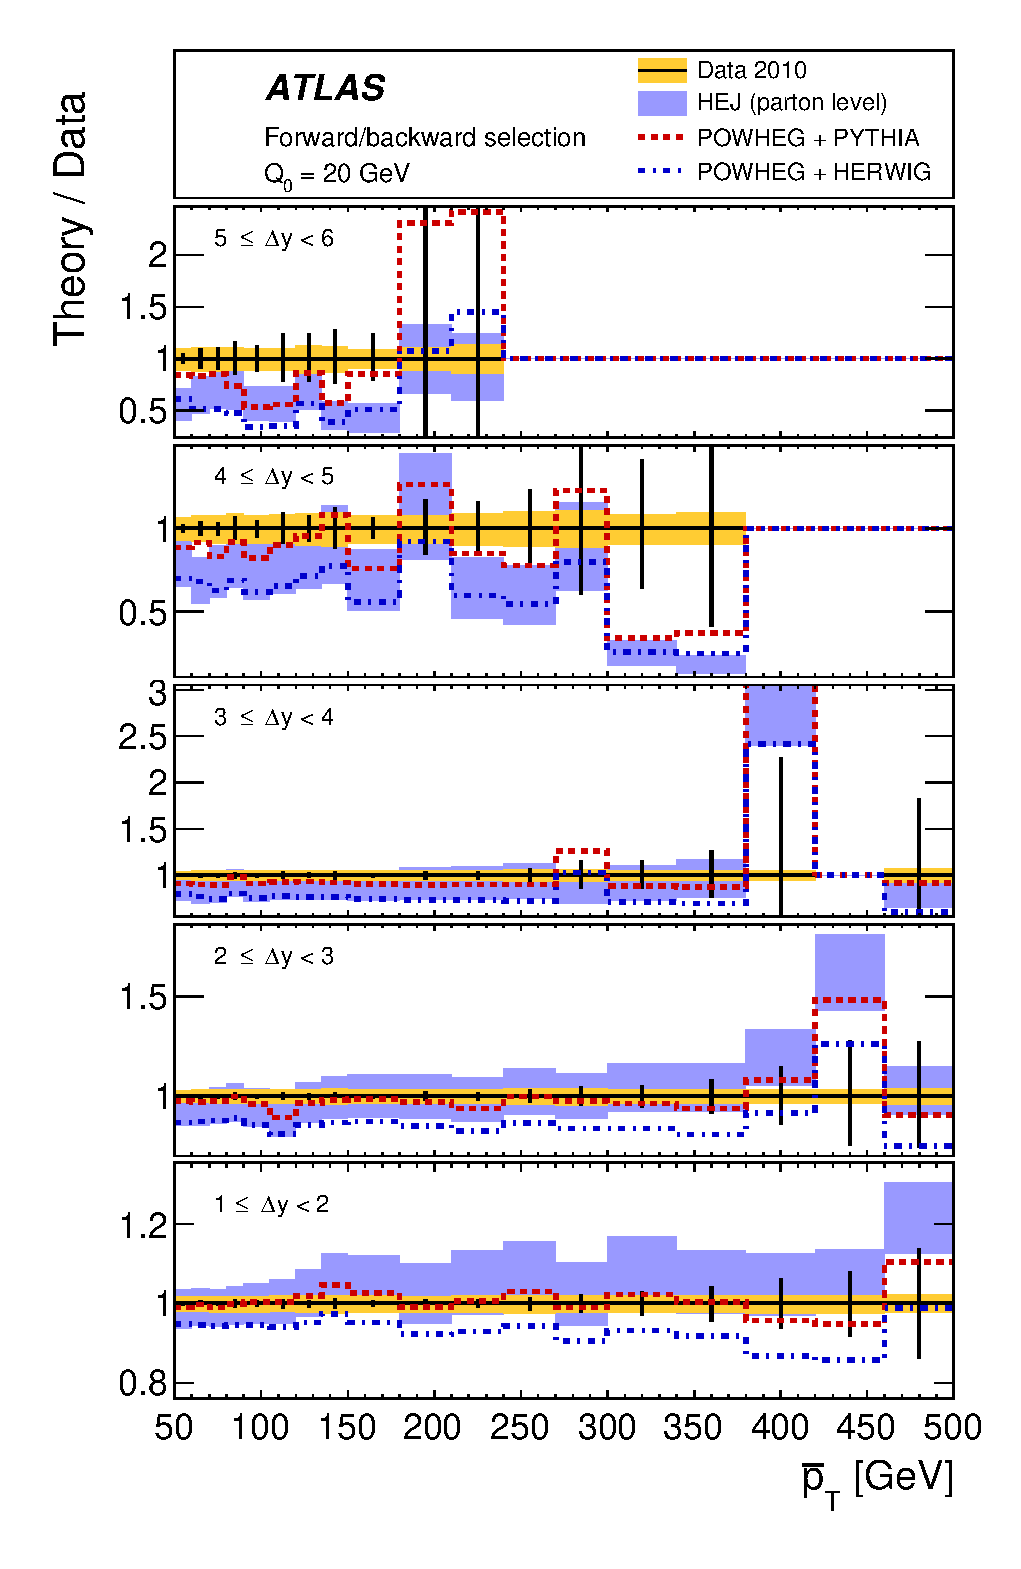
\includegraphics[width=\textwidth]{figures/GBJ1/FinalData/GF_SelB_pT_ratio.eps}
        \end{subfigure}%
\caption[Gap fraction as a function of \ptb{} for forward backward selection]{ 
(a) Gap fraction as a function of \ptb{} for various \dy{} slices for the forward backward selection. 
(b) Ratio between the theoretical predictions and data.
\label{GBJ1:pTSelB}}
\end{figure}

\begin{figure}
\centering
        \begin{subfigure}[b]{0.5\textwidth}
                \centering
                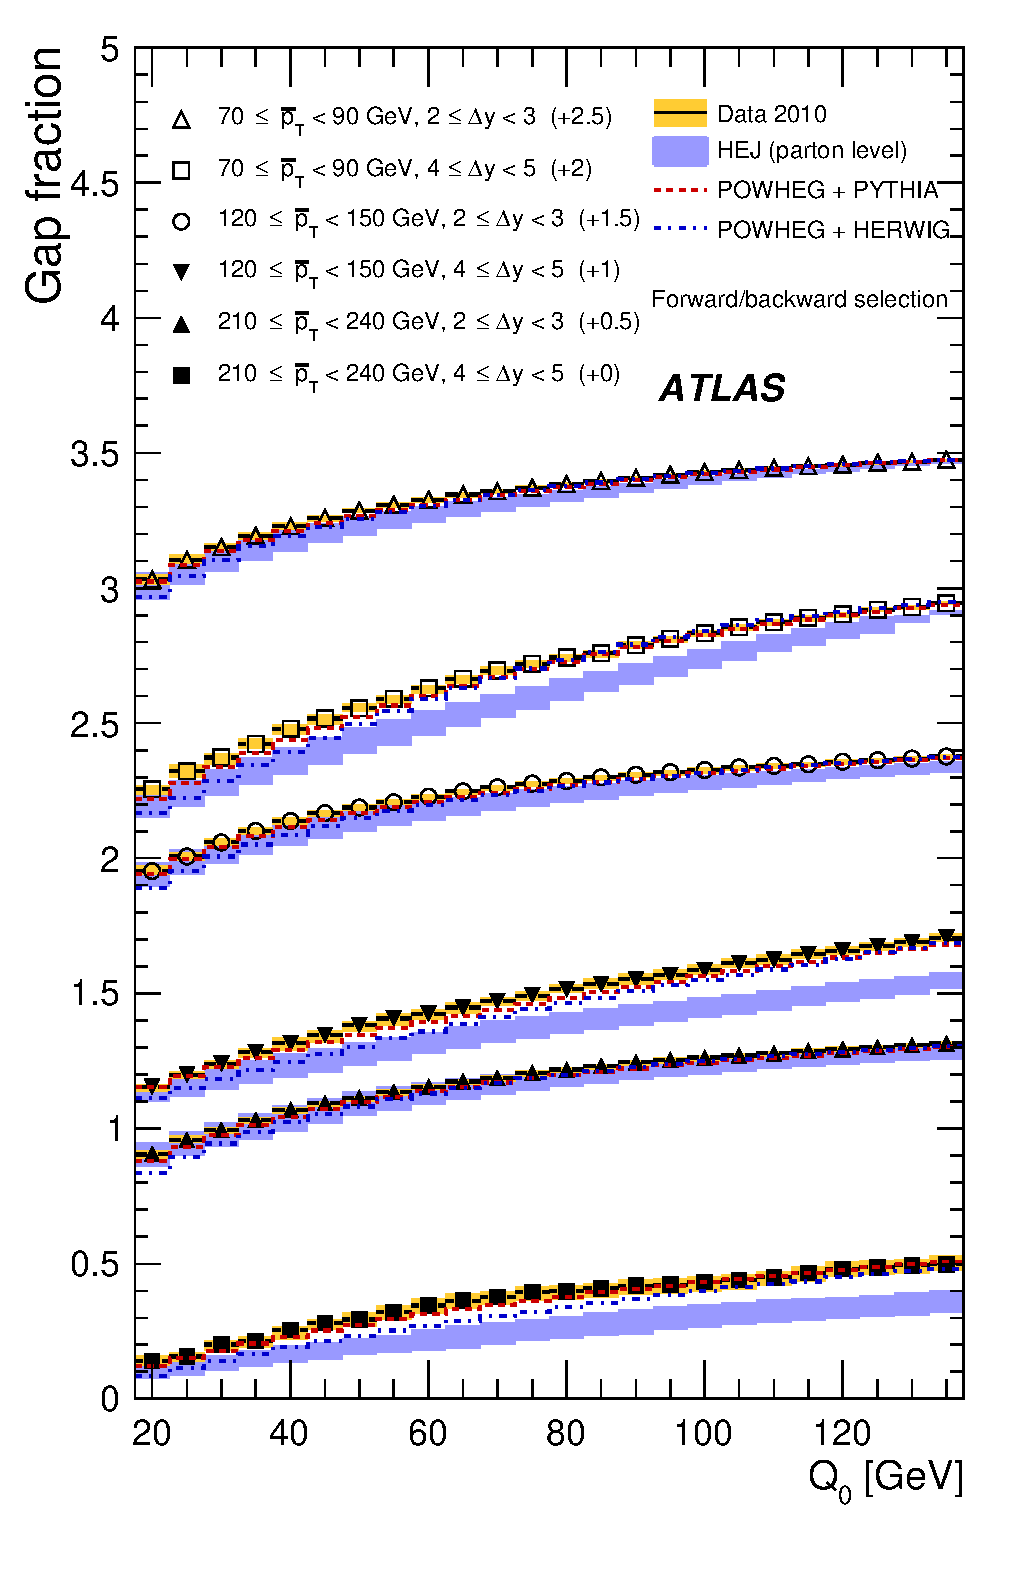
\includegraphics[width=\textwidth]{figures/GBJ1/FinalData/GF_SelB_Q0.eps}
        \end{subfigure}%
        \begin{subfigure}[b]{0.5\textwidth}
                \centering
                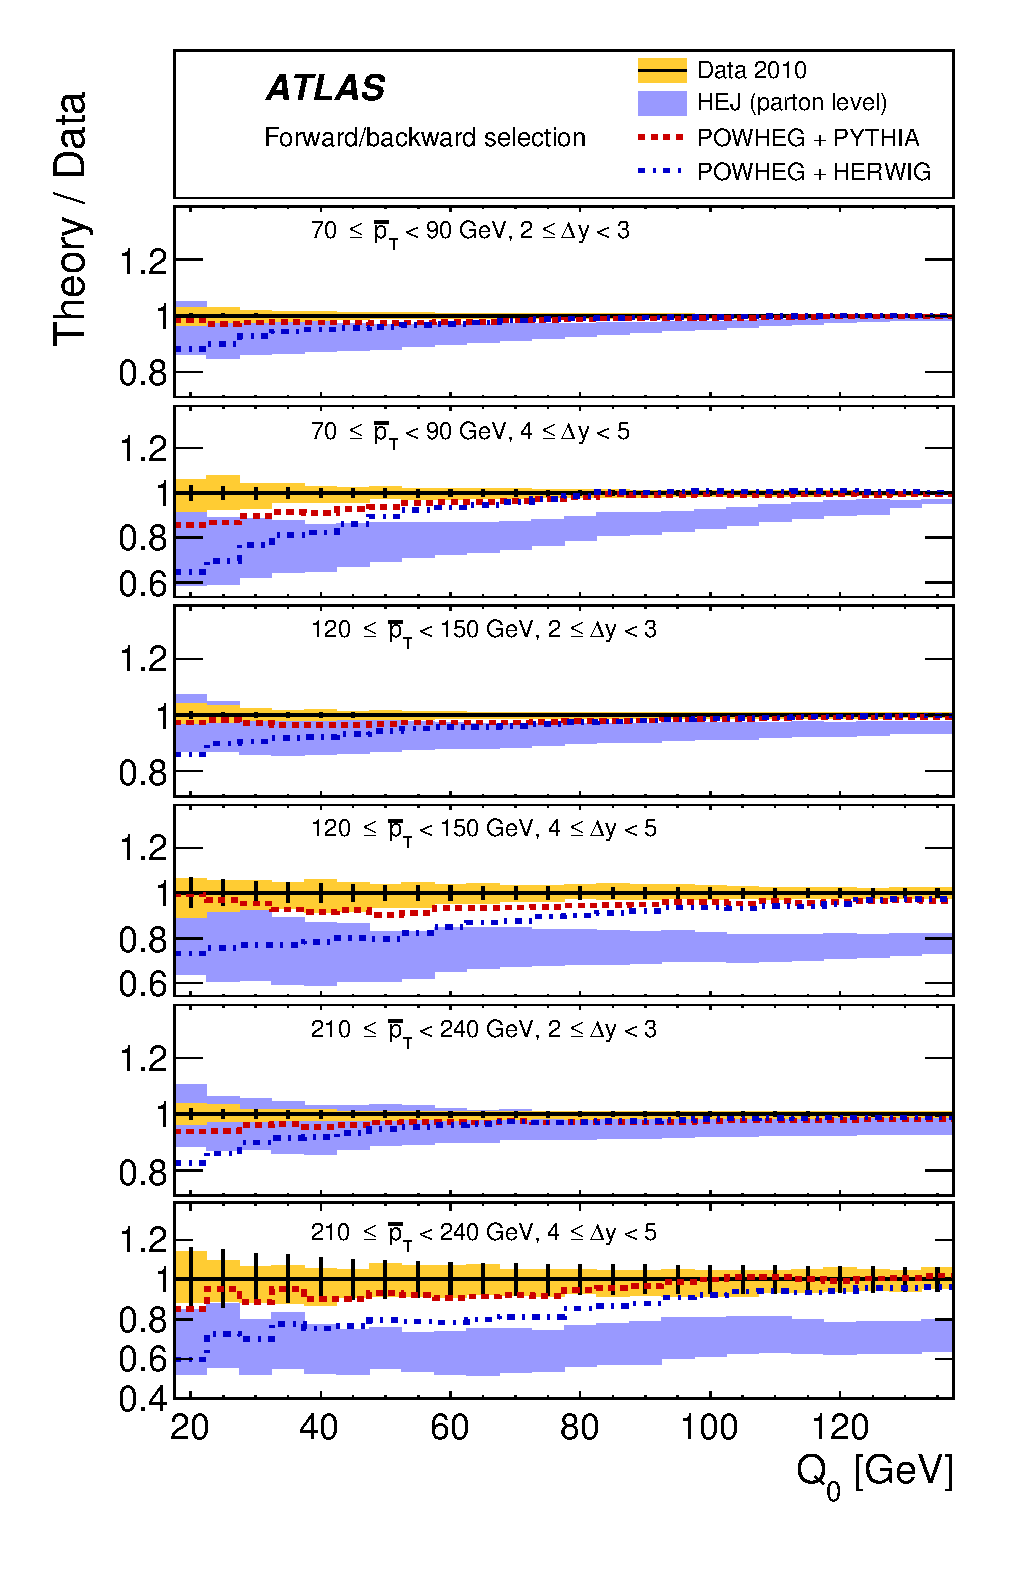
\includegraphics[width=\textwidth]{figures/GBJ1/FinalData/GF_SelB_Q0_ratio.eps}
        \end{subfigure}%
\caption[Gap fraction as a function of \qz{} for forward backward selection]{ 
(a) Gap fraction as a function of \qz{} for various \dy{} and \ptb{} slices for the forward backward selection. 
(b) Ratio between the theoretical predictions and data. 
\label{GBJ1:Q0SelB}}
\end{figure}


\begin{figure}
\centering
        \begin{subfigure}[b]{0.5\textwidth}
                \centering
                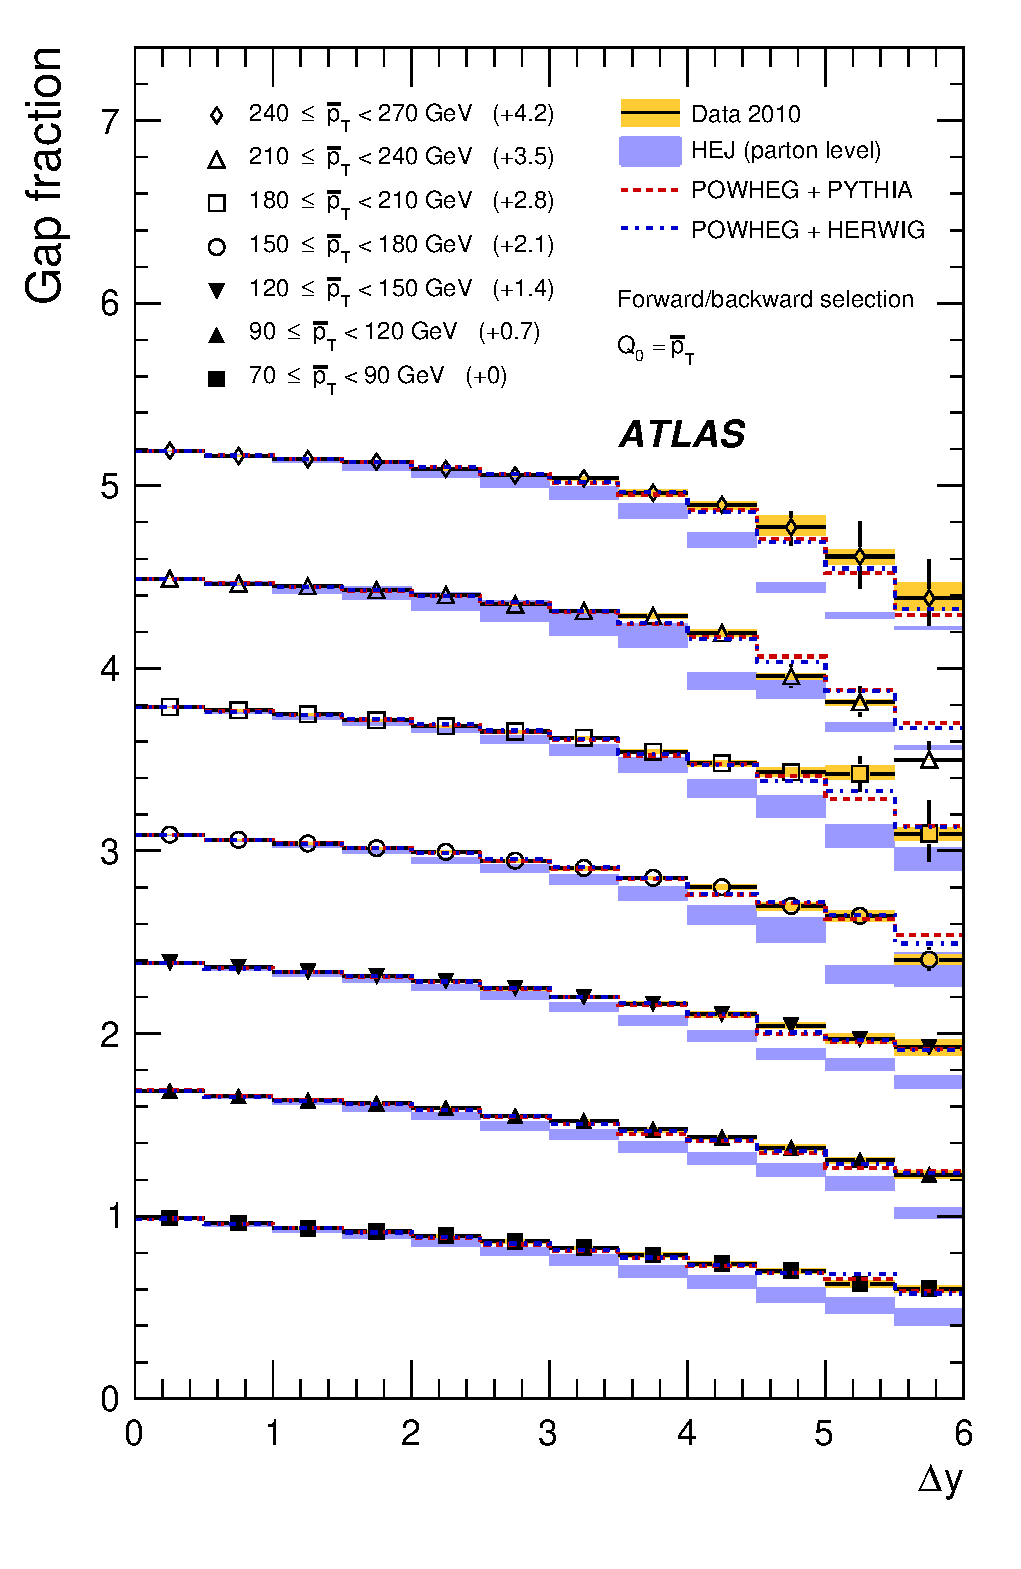
\includegraphics[width=\textwidth]{figures/GBJ1/FinalData/GF_SelB_dY_Q0pTbar.eps}
        \end{subfigure}%
        \begin{subfigure}[b]{0.5\textwidth}
                \centering
                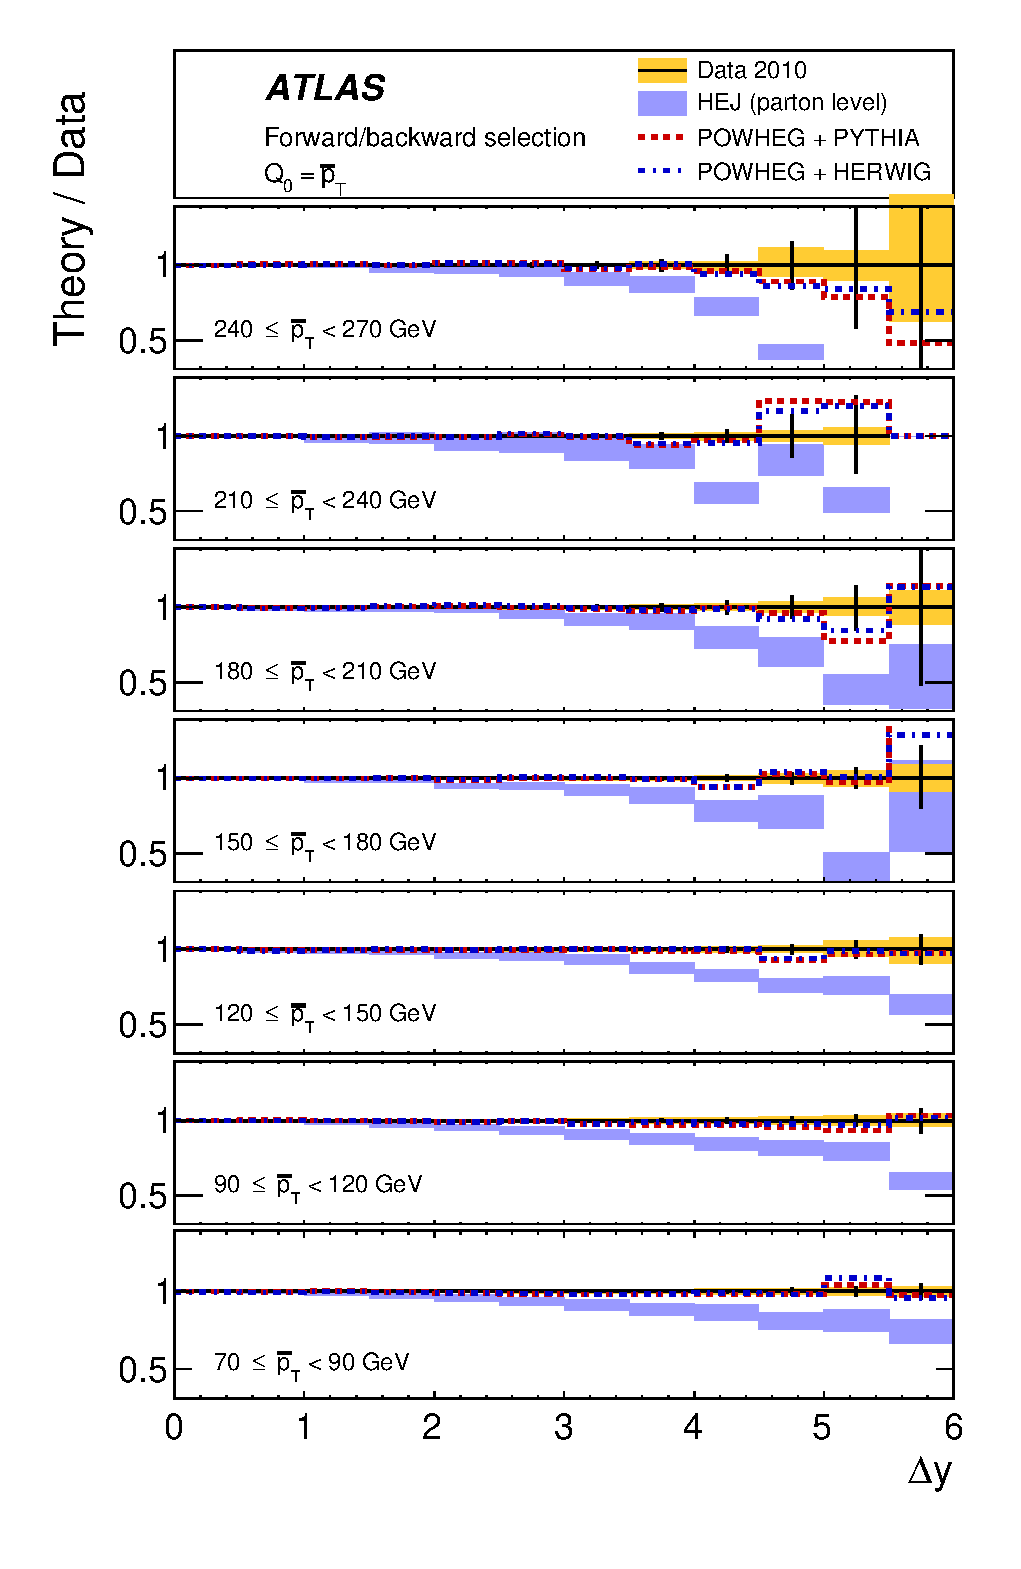
\includegraphics[width=\textwidth]{figures/GBJ1/FinalData/GF_SelB_dY_Q0pTbar_ratio.eps}
        \end{subfigure}%
\caption[Gap fraction as a function of \dy{} for forward backward selection and variable \qz{}]{ 
(a) Gap fraction as a function of \dy{} for various \ptb{} slices for the forward backward selection with veto scale set as \ptb{}. 
(b) Ratio between the theoretical predictions and data. 
\label{GBJ1:pTSelBQ0}}
\end{figure}

